% !TeX spellcheck = en_GB 
\section{Validation}
In order to validate our analytical models we compare its predictions against both simulation results and physical tensile tests.
While the physical tests constitute the final arbiter on the matter,
our resources for performing physical tests are limited.
Simulations can easily be performed by running a script for multiple days without user interaction.
Given that the simulations make use of the same material properties which were acquired from tensile tests performed by Ultimaker,
the simulations can teach us about the validity of the homogeneity assumptions in the analytical models.
Moreover, the physical test results are afflicted with a spread in manufacturing inaccuracies.
The simulations can therefore enrich the understanding we gain from physical experiments.




% !TeX spellcheck = en_GB 
\subsection{Simulation}
In order to simulate interlocking structures with a range of design parameters we automatically generate an INP file in Abaqus CAE (2020) using a script.
Solving the INP file gives us the force-displacement graph, from which we can determine the ultimate tensile strength.
In order to simulate accurately we used the stress-strain curves from tensile tests on the base materials printed flat on the build plate as the plasticity in tabular form.
The simulations were performed in the Abaqus/Explicit solver where Dynamic, Explicit procedure step was used with the mass scaling factor of $10^7$,
using geometric nonlinearity and general contact (explicit) to disregard friction for simplicity.

The repeating nature of the interlocking patterns was captured by modelling half of the unit cell and apply symmetry constraints to the sides, top and bottom.
The model was meshed using C3D8R hexahedral elements of $\pm\SI{75}{\micro\meter}$.

A grid search was used to measure the influence on the ultimate strength along each of the design variables $\wb (,\va, \hc)$, along with the total length $L$.
The search space was therefore 4D and 2D for the straight and diagonal design respectively.
In order to estimate the optimum we fit a smooth response surface to these data points using a radial basis function (RBF) network\cite{Dinh2002},
where a smoothness of $\lambda=1$ produces satisfactory results.


\subsubsection{Straight}
In order to prevent stress concentrations and adhere to manufacturing accuracy, the vertical edges of the straight design were rounded with $r=\SI{0.15}{\milli\meter}$;
see \cref{fig:sim_straight_model}.
We performed two rounds of hypersurface fitting on grid search; the second round was in a zoomed in region and with elements of $\pm\SI{50}{\micro\meter}$.

Newton's method was used to determine the optimum, starting from the best sampled point.
This step only considered the dimensions $\wb$ and $\va$, because $\lmax$ is given and $\hf$ has to be an integer multiple of $\hmin$.
It's unlikely the optimum of the fitted hypersurface would be on a different integer multiple of $\hmin$.
The resulting hypersurfaces are visualized in \cref{fig:simulation_results_straight}.
The obtained optima are shown in \cref{tab:sim_straight_optima}.

We compare the results of round 1 to our analytical model by adjusting the analytical model to capture the inaccurate Z strength used in the simulations:
$\sigmafailz{m} := \sigmafail{m}$.
See \cref{fig:ana_sim_accuracy_straight}.
We then observe that our analytical model on average predicts only \SI{7.8}{\percent} higher ultimate strength values than then the FEM simulations, with a standard deviation of \SI{16.2}{\percent}.

\begin{figure}
	\centering
	\setlength{\figheight}{.32\columnwidth}
	\begin{subfigure}[B]{.6\columnwidth}
		\centering
		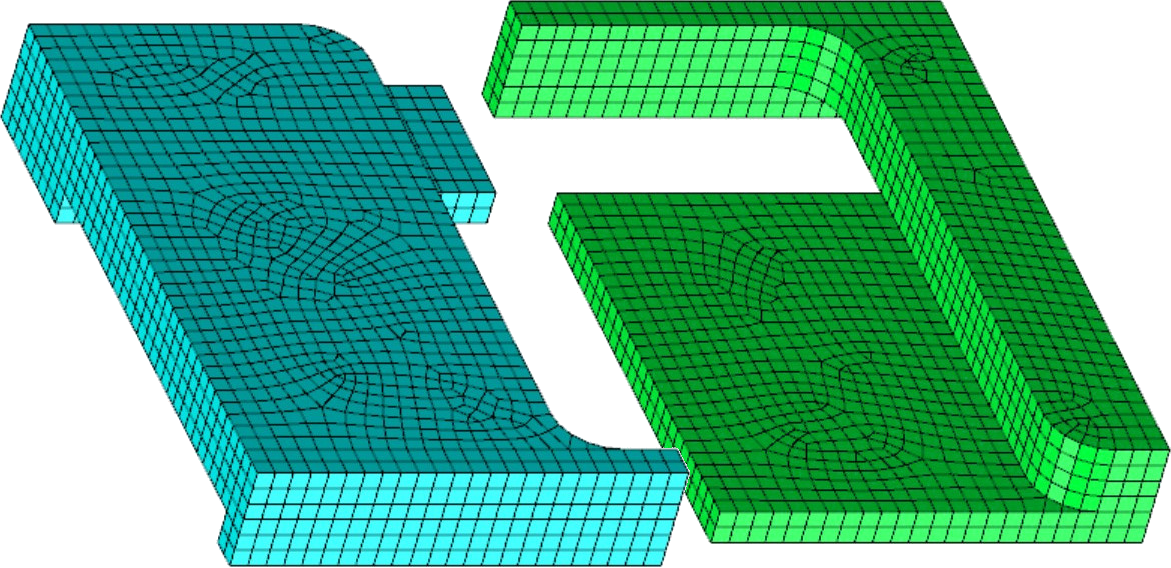
\includegraphics[height=\figheight]{sources/simulation/mesh-straight.png}
		\caption{Straight}
	\end{subfigure}
\hspace{-.5cm}
	\begin{subfigure}[B]{.39\columnwidth}
		\centering
		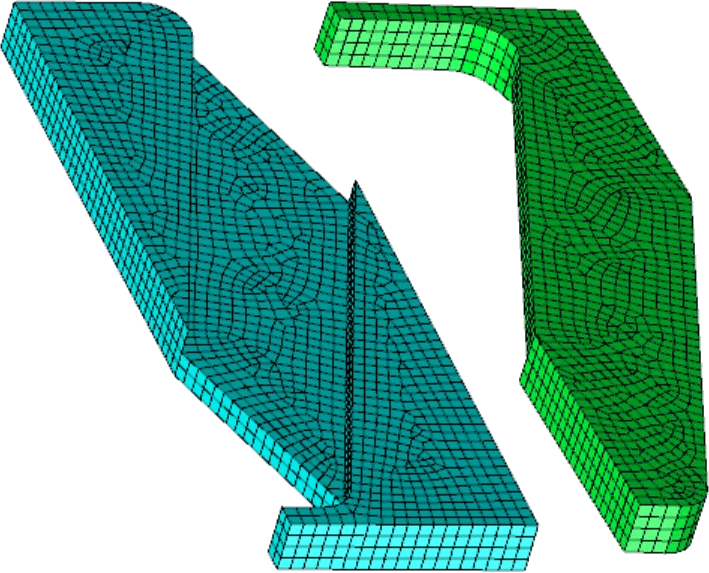
\includegraphics[height=\figheight]{sources/simulation/mesh-diagonal.png}
		\caption{Diagonal}
	\end{subfigure}
	\caption{Example simulation meshes. The diagonal mesh is half a unit cell.}
	\label{fig:sim_straight_model}
\end{figure}



\begin{figure*}
	\centering
	\begin{subfigure}[B]{.49\columnwidth}
		\centering
		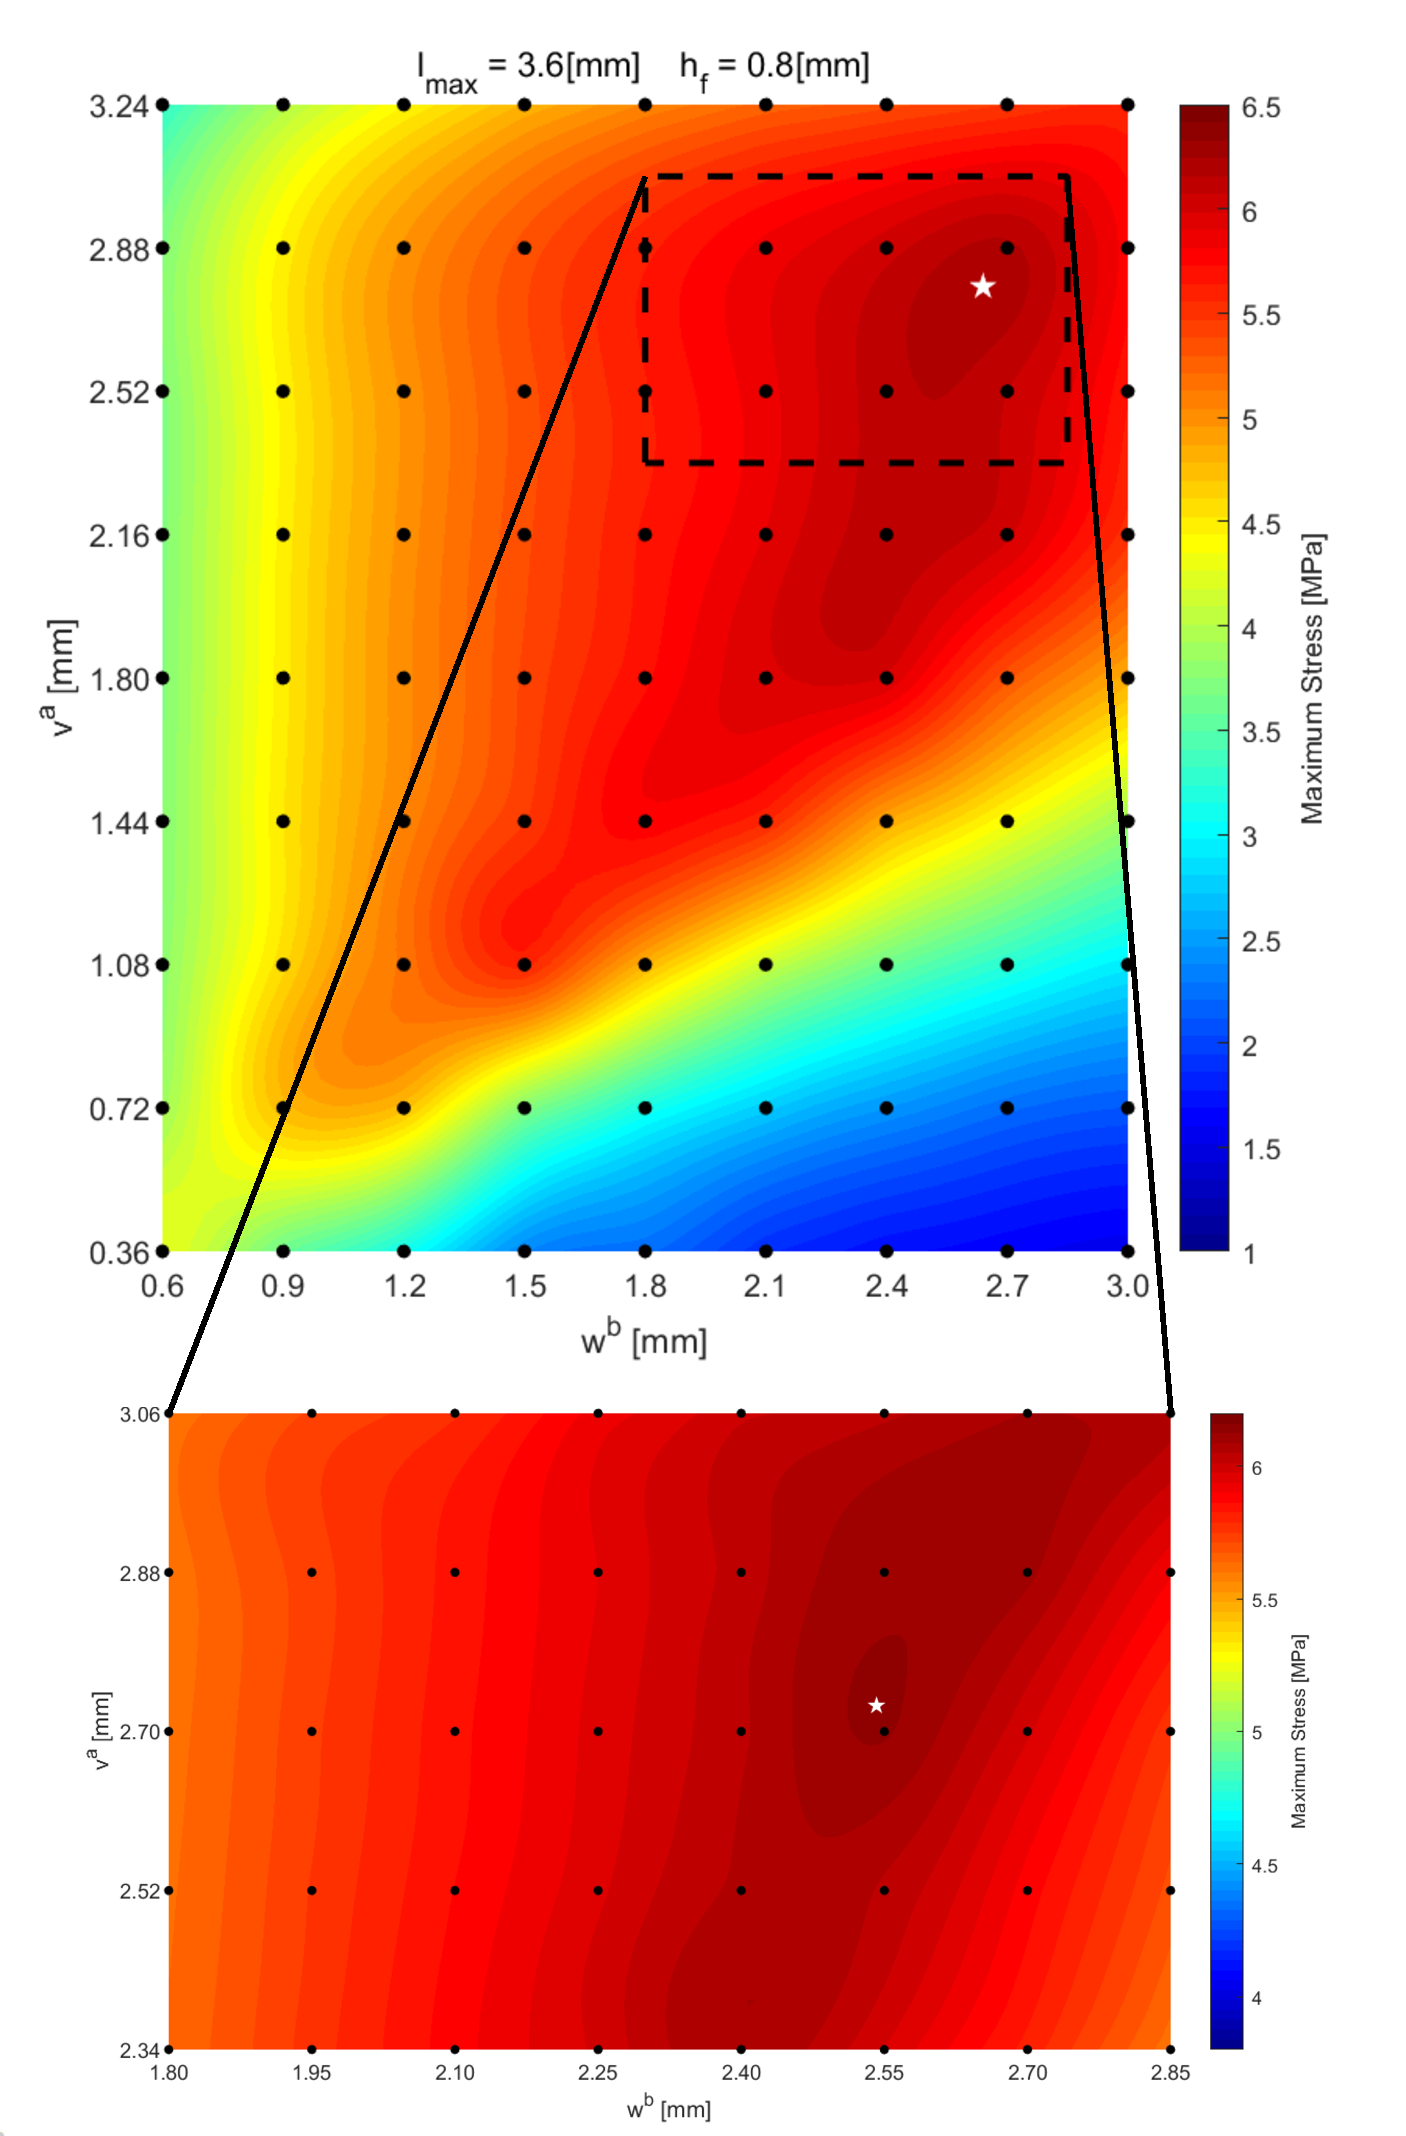
\includegraphics{sources/simulation/r12-lmax3.6.pdf}
		\caption{$\lmax=\SI{3.6}{\milli\meter}; \hf=\SI{0.8}{\milli\meter}$}
	\end{subfigure}
	\begin{subfigure}[B]{.49\columnwidth}
		\centering
		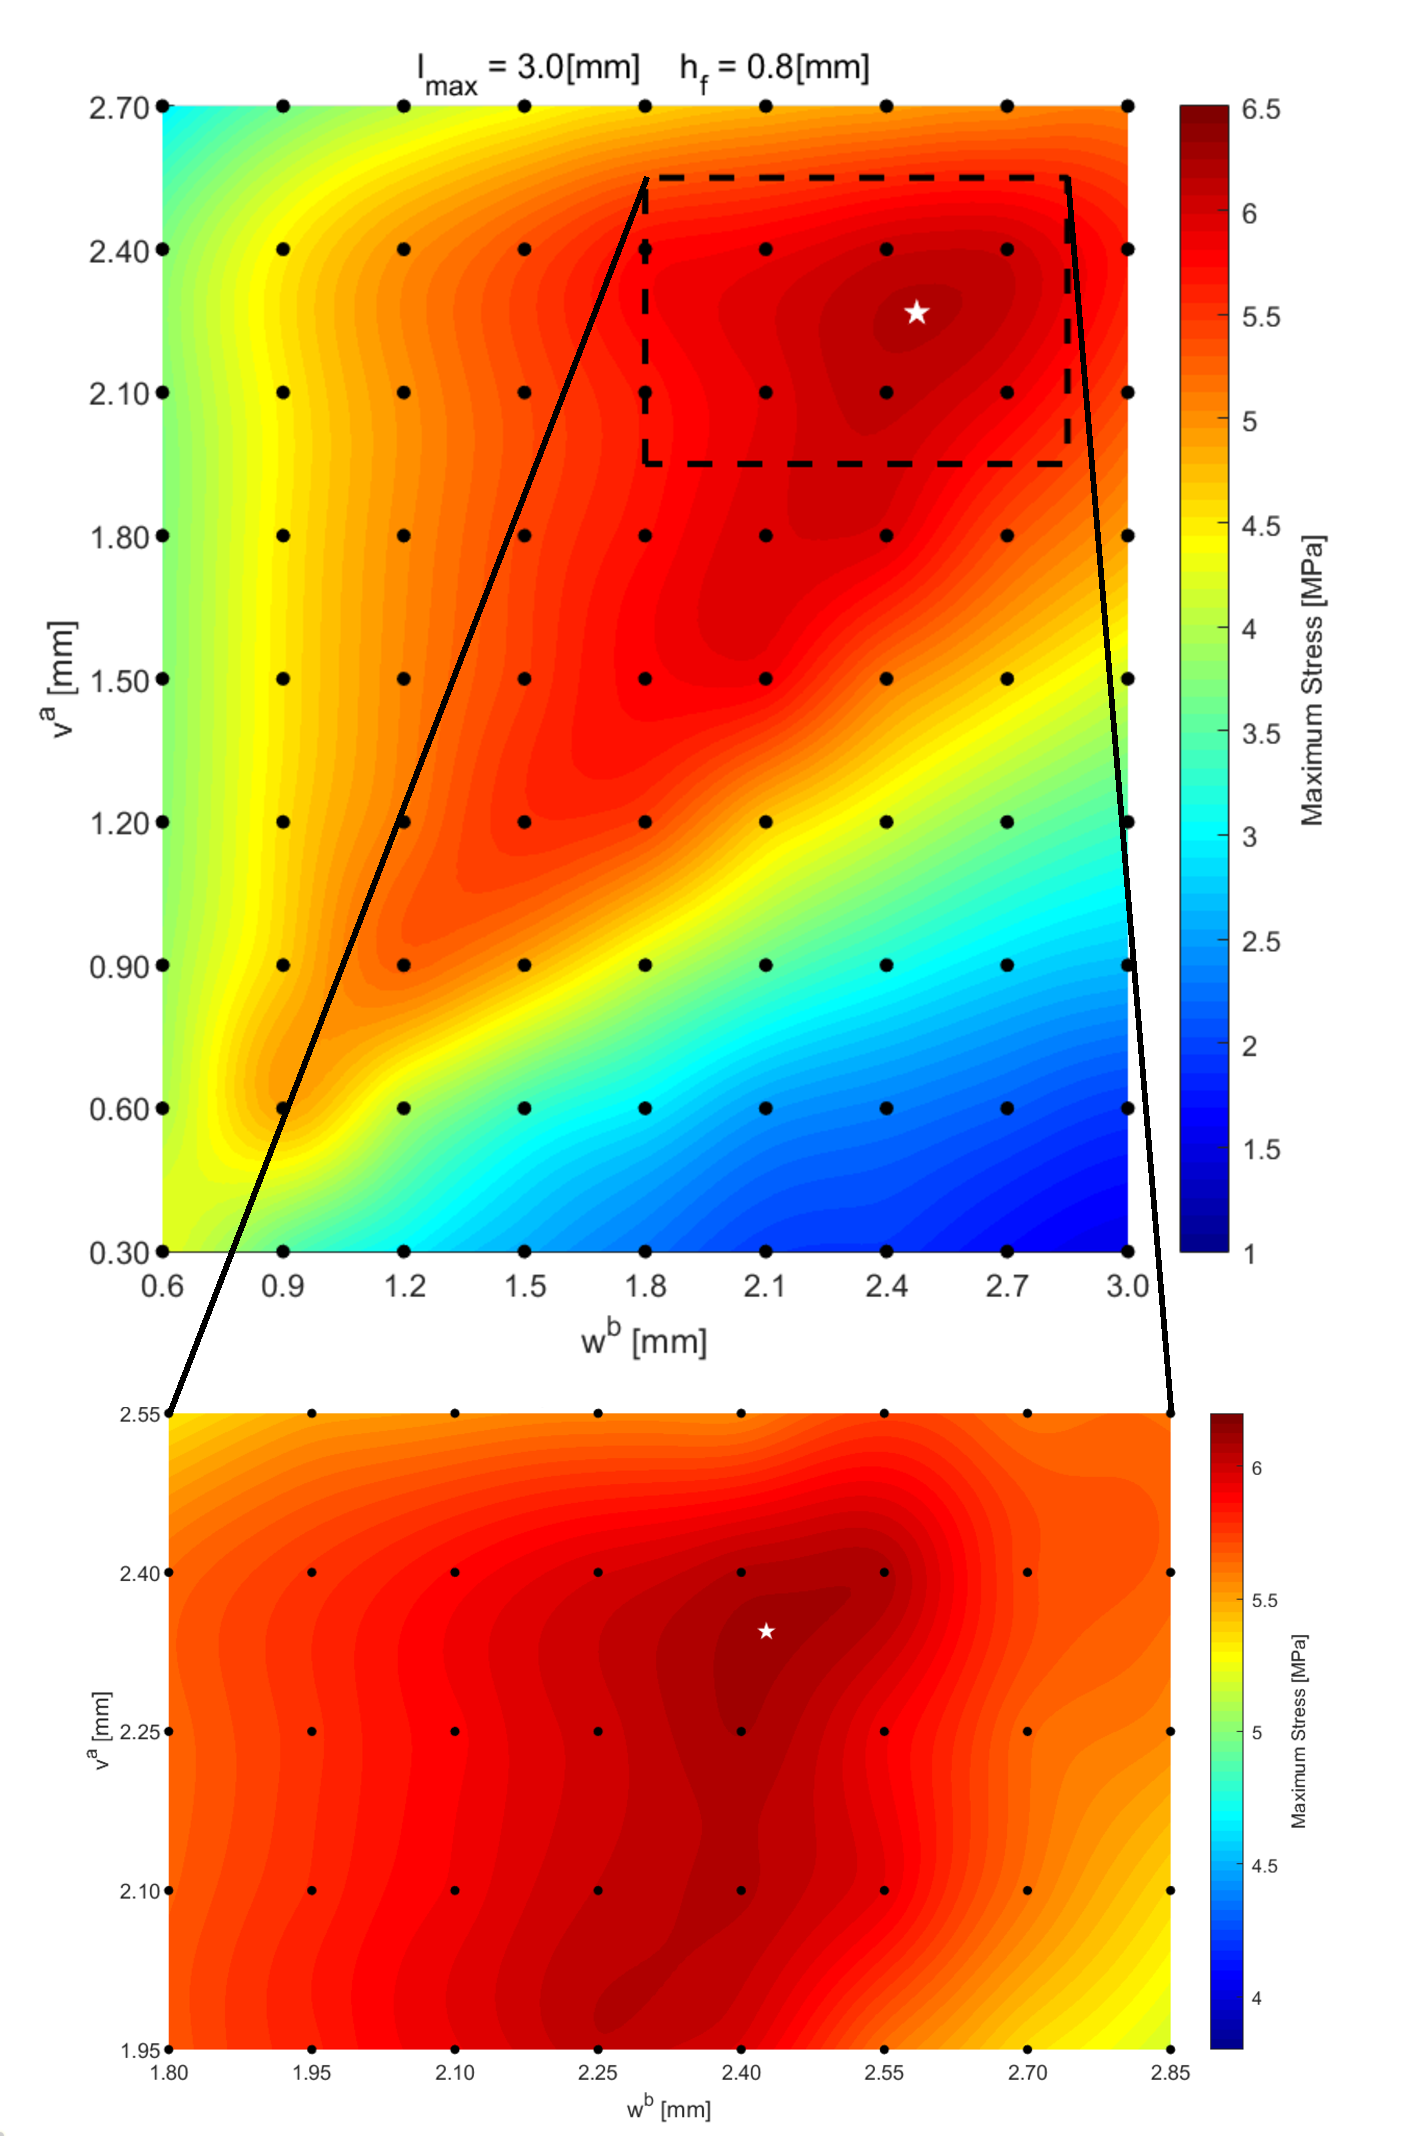
\includegraphics{sources/simulation/r12-lmax3.0.pdf}
		\caption{$\lmax=\SI{3.0}{\milli\meter}; \hf=\SI{0.8}{\milli\meter}$}
	\end{subfigure}
	\begin{subfigure}[B]{.49\columnwidth}
		\centering
		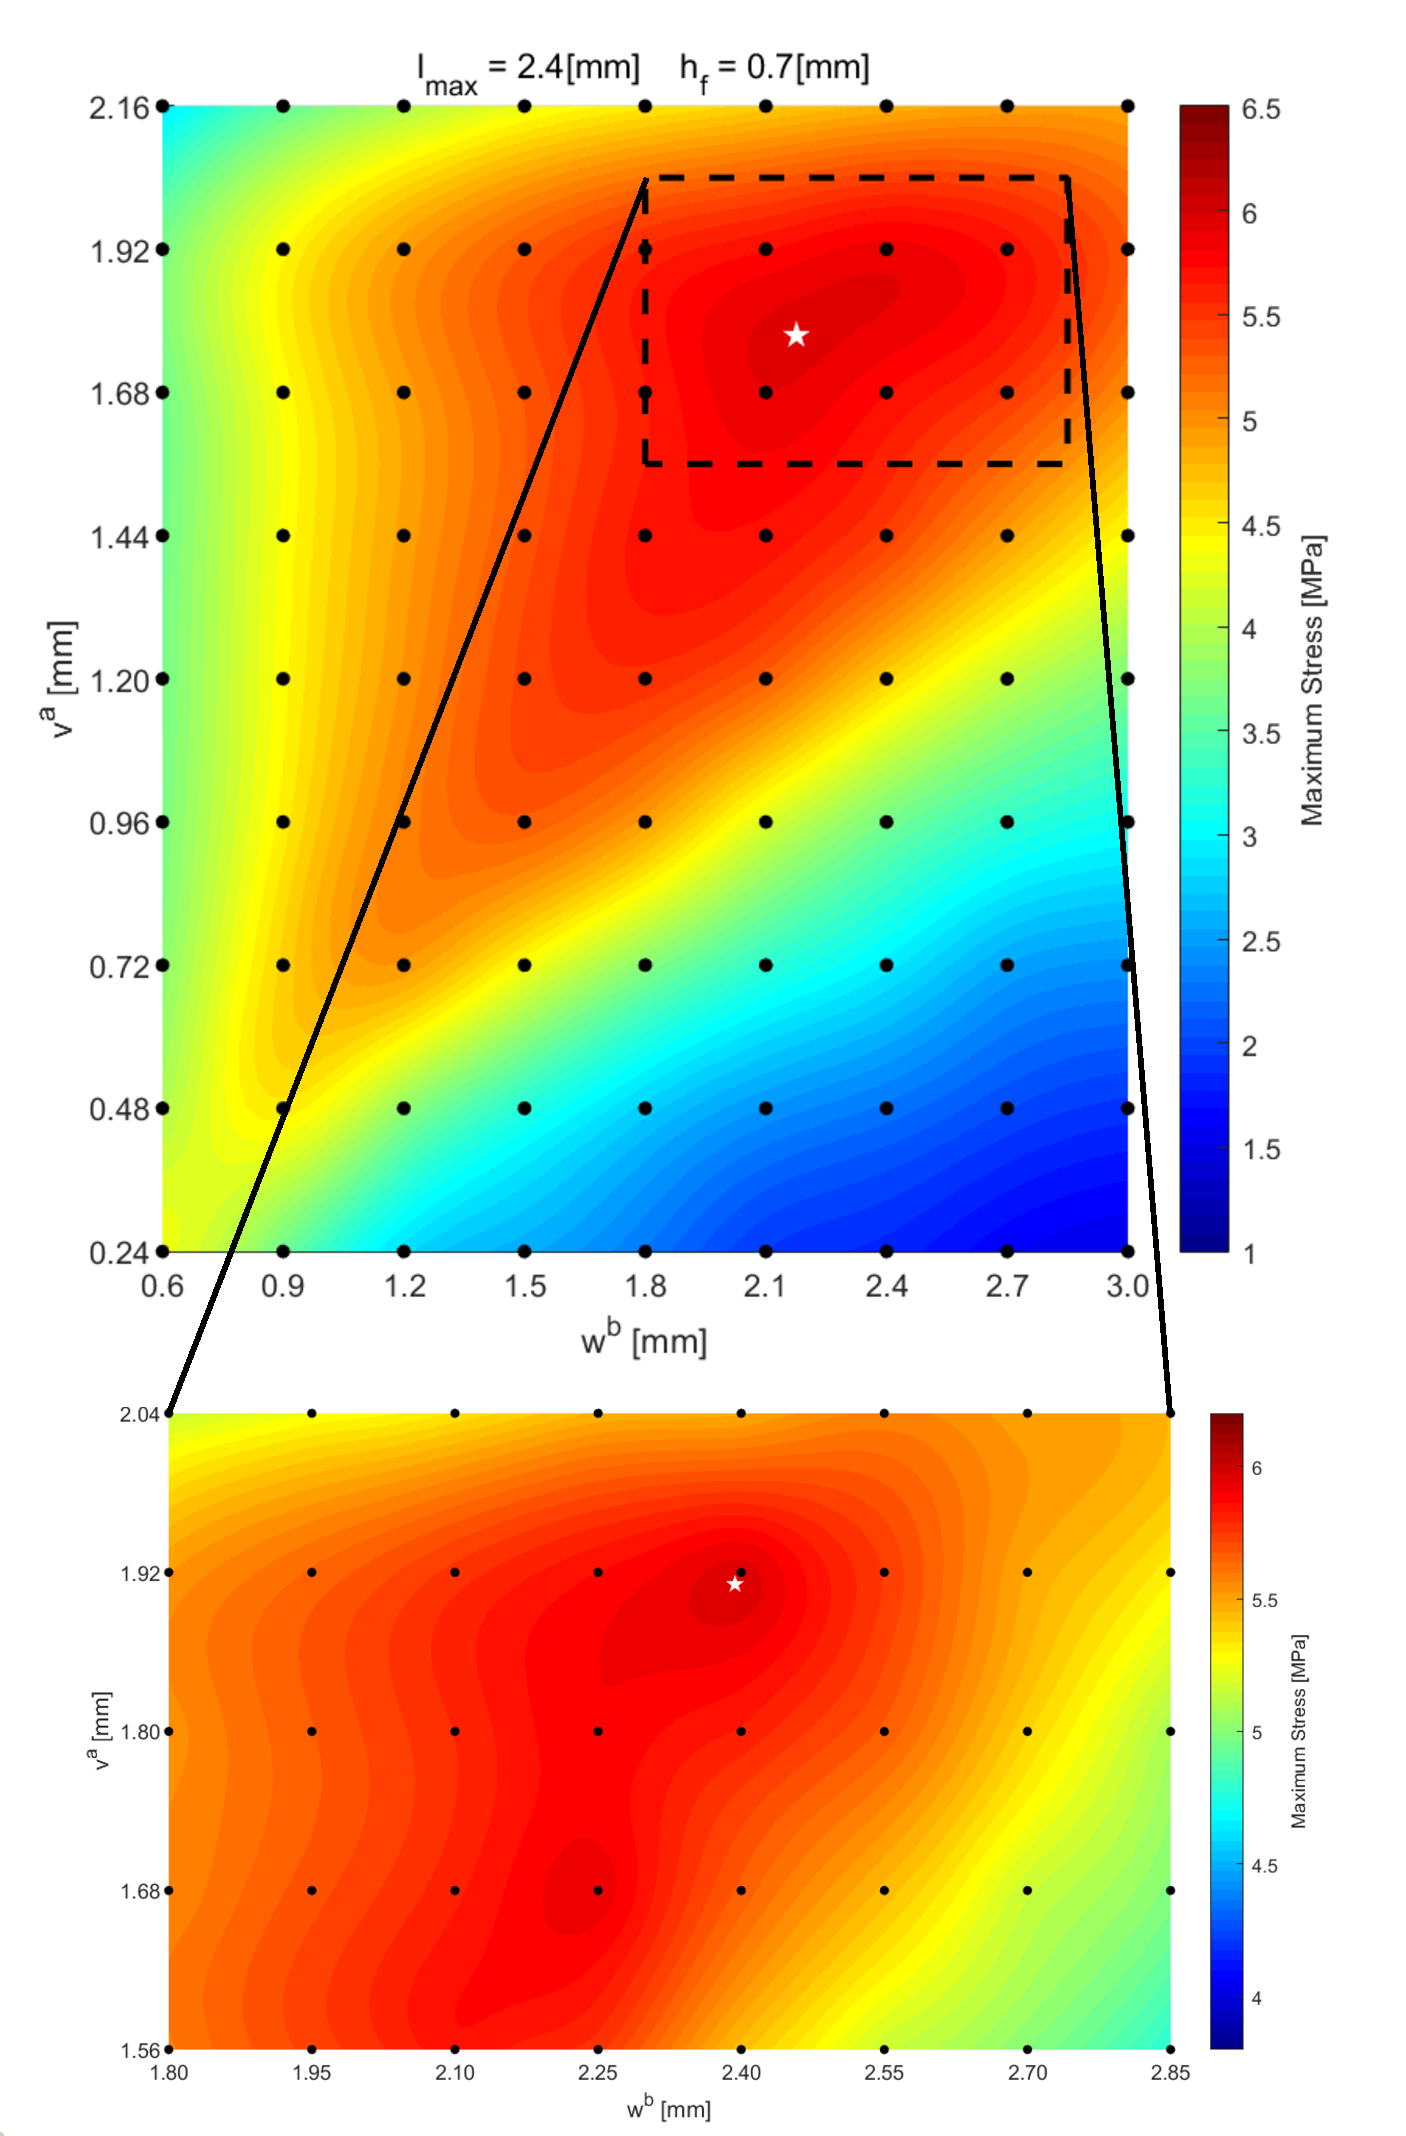
\includegraphics{sources/simulation/r12-lmax2.4.pdf}
		\caption{$\lmax=\SI{2.4}{\milli\meter}; \hf=\SI{0.7}{\milli\meter}$}
	\end{subfigure}
	\begin{subfigure}[B]{.49\columnwidth}
		\centering
		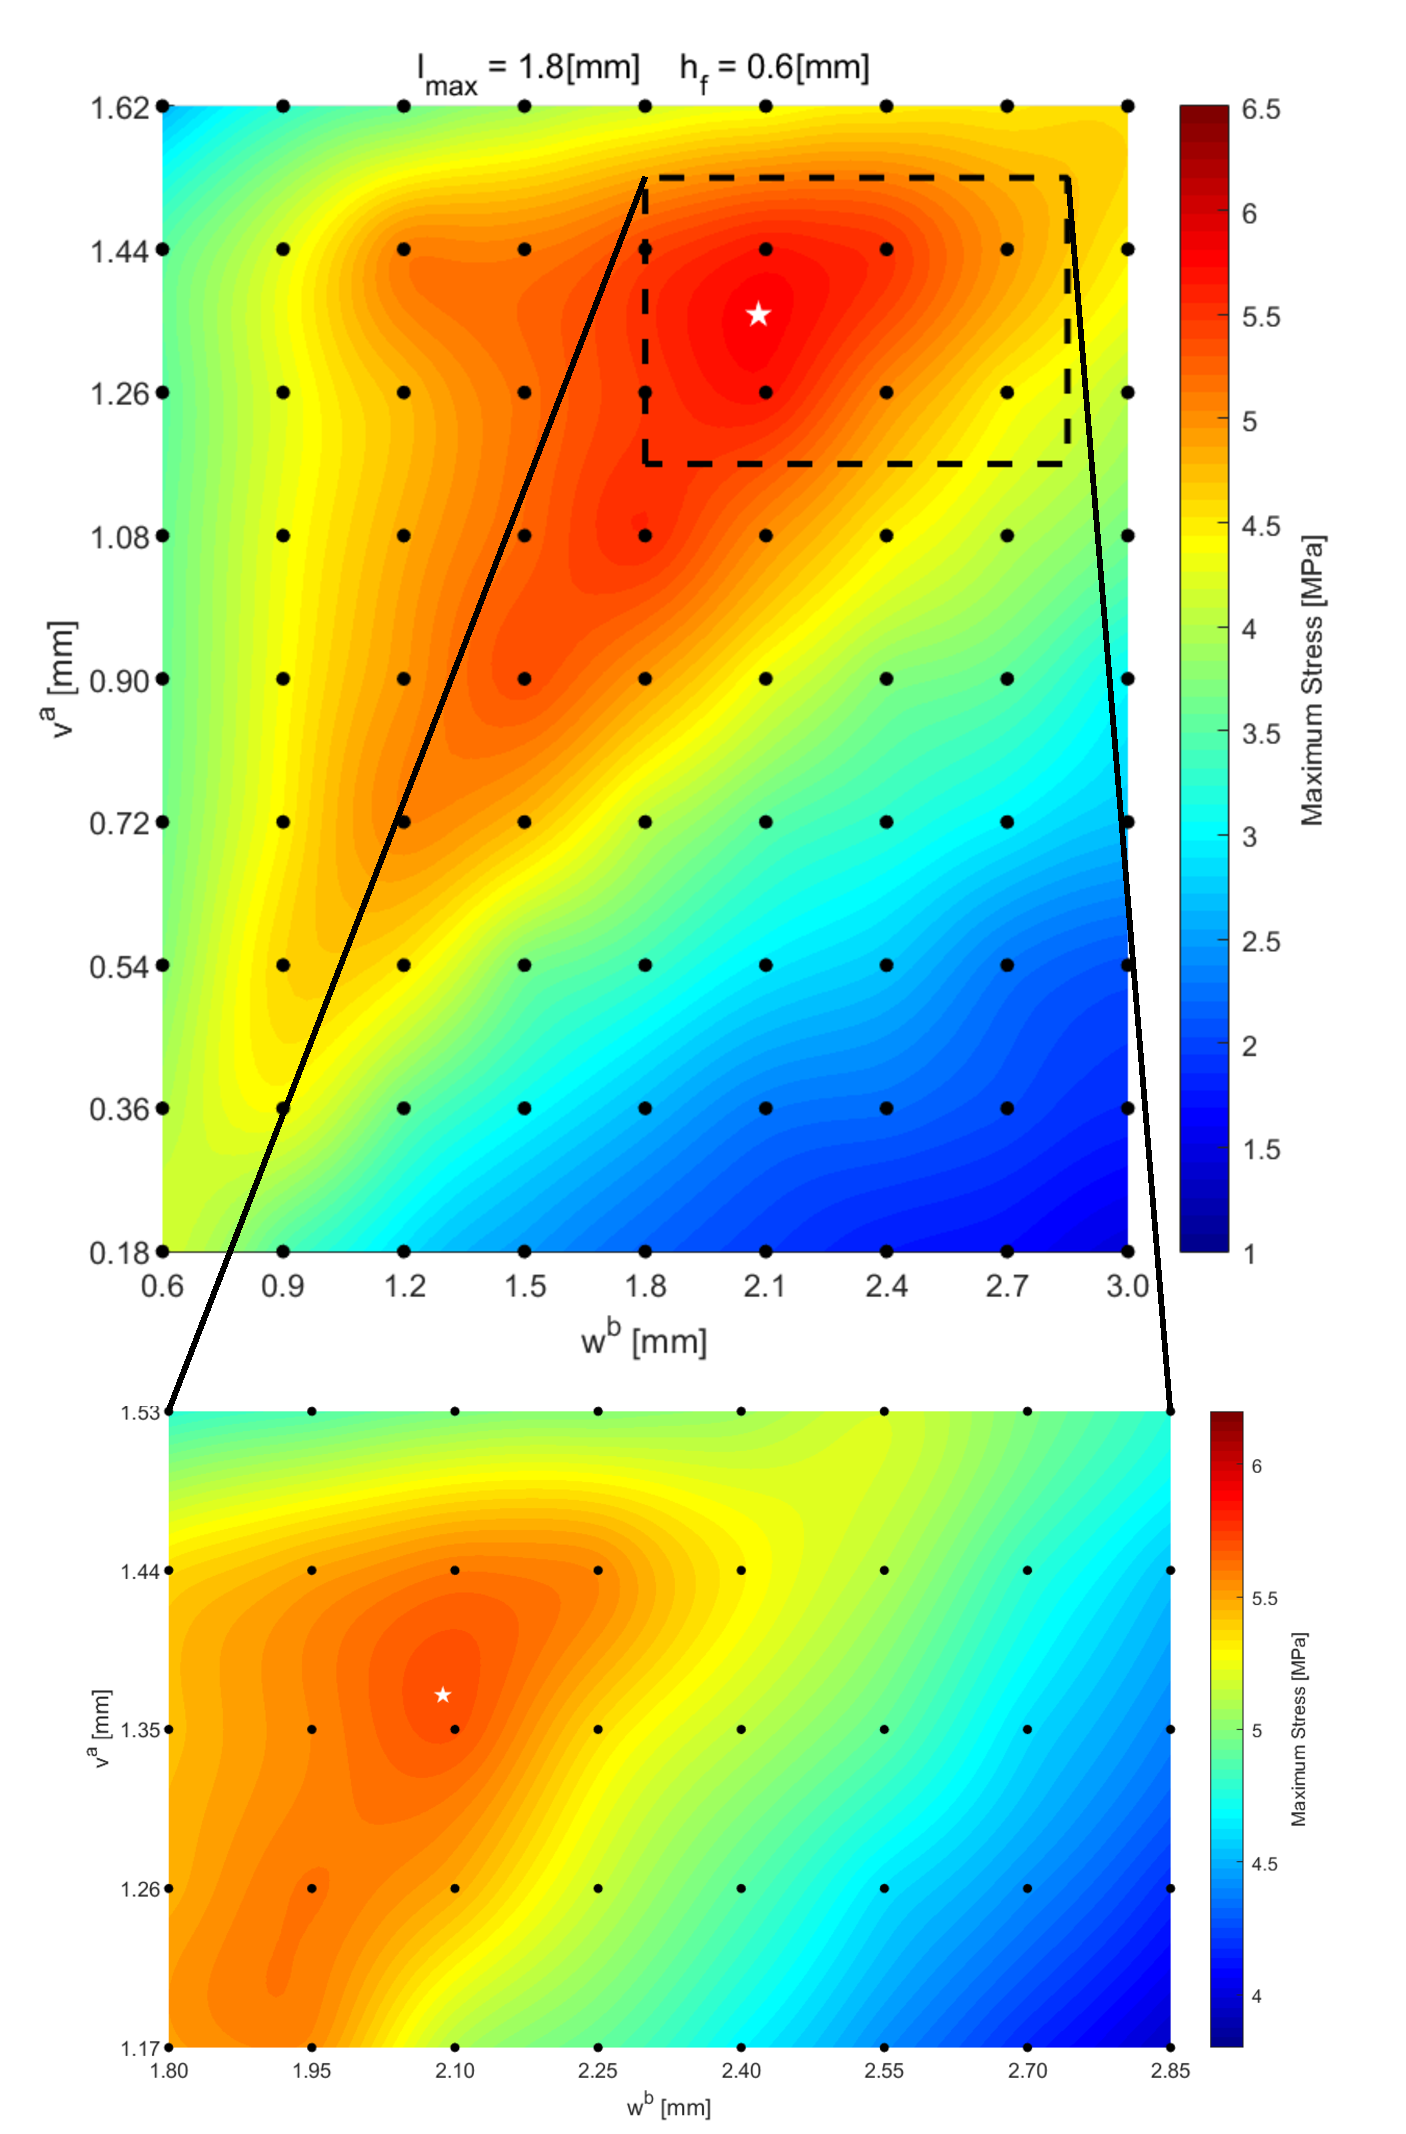
\includegraphics{sources/simulation/r12-lmax1.8.pdf}
		\caption{$\lmax=\SI{1.8}{\milli\meter}; \hf=\SI{0.6}{\milli\meter}$}
	\end{subfigure}
	\caption{2D slices of the 4D simulation results and fitted hypersurface for the straight design. Sampled data points in black, optimum in white.}
	\label{fig:simulation_results_straight}
\end{figure*}

\begin{table}
	\caption{Optimal designs according to the hypersurface fitted to the FEM simulations for the second round of the straight model and for the diagonal model.}
	\label{tab:sim_straight_optima}
	\begin{tabular}{ll|llll}
		&$\lmax$ (\si{\milli\meter})             & 3.6 & 3.0 & 2.4 & 1.8 \\
		\hline
		\multirow{4}{*}{\rotatebox[origin=c]{90}{straight}}
		&$\sigma_\text{max}$ (\si{\mega\pascal}) & \bf 6.11 & \bf 6.03 & \bf 5.81 & \bf 5.53 \\
		&$\hf$ (\si{\milli\meter})               & 0.8 & 0.8 & 0.7 & 0.6 \\
		&$\wb$ (\si{\milli\meter})               & 2.54 & 2.35 & 2.22 & 2.01 \\
		&$\va$ (\si{\milli\meter})               & 2.82 & 2.27 & 1.84 & 1.36 \\
		\hline
		\multirow{2}{*}{\rotatebox[origin=c]{90}{diag}}
		&$\sigma_\text{max}$ (\si{\mega\pascal}) & \bf 6.30 & \bf 6.37 & \bf 5.86 & \bf 4.69 \\
		&$\wb$ (\si{\milli\meter})               & 1.21 & 1.19 & 1.18 & 1.04 \\
		\end
		{tabular}
\iffalse
	\begin{tabular}{l|llllllll}
		Round & 1 & 2 & 1 & 2 & 1 & 2 & 1 & 2 \\
		\hline
		$\lmax$ (\si{\milli\meter}) & 3.6 & 3.6 & 3.0 & 3.0 & 2.4 & 2.4 & 1.8 & 1.8\\
		$\hf$ (\si{\milli\meter}) & 0.8 & 0.8 & 0.8 & 0.8 & 0.7 & 0.7 & 0.6 & 0.6 \\
		$\wb$ (\si{\milli\meter}) & 2.58 & 2.54 & 2.42 & 2.35 & 2.18 & 2.22 & 2.05 & 2.01\\
		$\va$ (\si{\milli\meter}) & 2.67 & 2.82 & 2.23 & 2.27 & 1.78 & 1.84 & 1.35 & 1.36 \\
		$\sigma_\text{max}$ (\si{\mega\pascal}) & 6.17 & 6.11 & 6.12 & 6.03 & 5.89 & 5.81 & 5.59 & 5.53
	\end{tabular}
\fi
\end{table}





\subsubsection{Diagonal}
Modelling the diagonal design in Abaqus can be quite cumbersome, since it doesn't natively support periodic boundary constraints.
Whereas this problem can be overcame in the straight design because it is symmetric,
the diagonal design is rotationally symmetric.
While a symmetry constraint can be used on the top and bottom, the two sides of the design are mirror images of each other, but also flipped vertically.

However, since the height of the beams is relatively low compared to their width we have observed that the stresses and strains are quite similar in the top and bottom.
If we model half of the diagonal cell by cutting it vertically and apply symmetry constraints to the sides,
the induced error is only approximately 10\% compared to simulating an interface consisting of two whole cells.
% small discontinuities



\begin{figure}
	\centering
	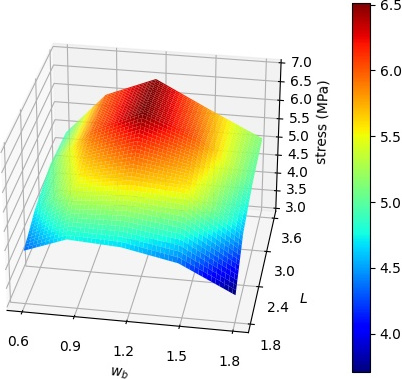
\includegraphics[width=.7\columnwidth]{sources/simulation/diagonal_sim_response.jpg}
	\caption{Diagonal results using linear interpolation between the simulation results.}
	\label{fig:sim_diagonal_model}
\end{figure}


The results of these simulations are shows in \cref{fig:sim_diagonal_model}.
The predictions from the analytical model can directly be compared to the simulation results, because the constraints on Z shear are not active.
See \cref{fig:ana_sim_accuracy_diagonal}.
The analytical model predicts only 0.4\% lower ultimate strength values on average with a standard deviation of 10\%.

%optimal designs table



\begin{figure*}
	\centering
	\setlength{\figheight}{.2\textwidth}
	\begin{subfigure}[B]{.7\textwidth}
		\centering
		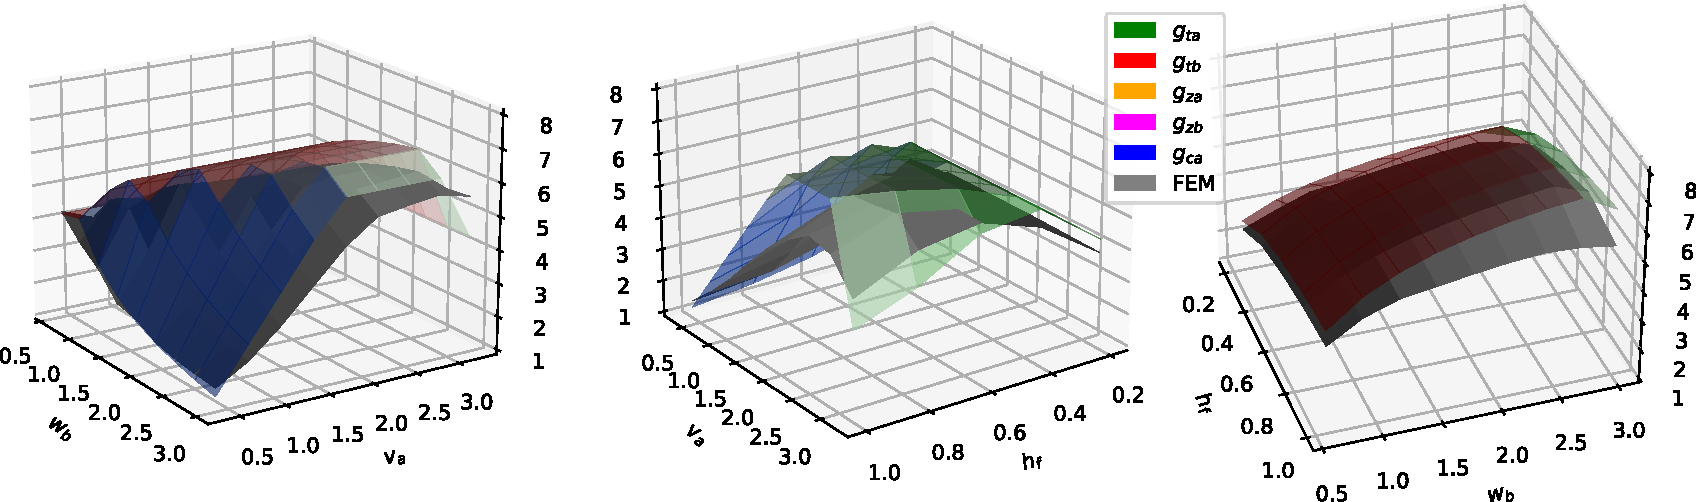
\includegraphics[height=\figheight]{sources/simulation/model_accuracy.pdf}
		\caption{Straight ITIM for $L=\SI{3.6}{\milli\meter}$}
		\label{fig:ana_sim_accuracy_straight}
	\end{subfigure}
	\hspace{-.5cm}
	\begin{subfigure}[B]{.29\textwidth}
		\centering
		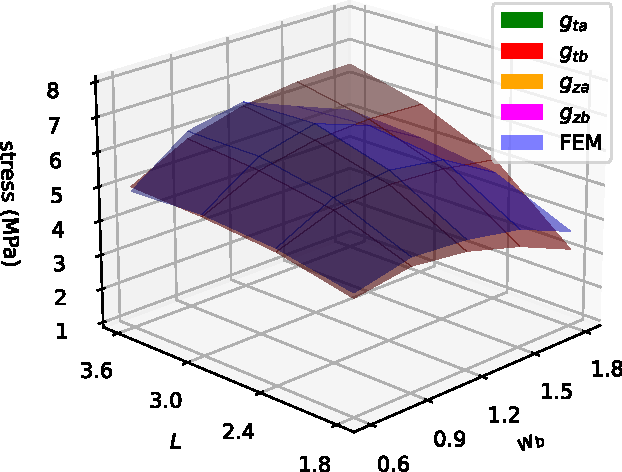
\includegraphics[height=\figheight]{sources/simulation/model_accuracy_diagonal.pdf}
		\caption{Diagonal ITIM for various values of $L$}
		\label{fig:ana_sim_accuracy_diagonal}
	\end{subfigure}
	\caption{Ultimate strength according to the analytical models and the simulation results. The analytical models follow roughly the same shape and same height as the simulation results. }
	\label{fig:ana_sim_accuracy}
\end{figure*}









\subsection{Physical experimental tests}
Tensile tests were performed on an Instron 3366 Universal Testing machine at \SI{5}{\milli\meter\per\minute}.
Prints were manufactured on a Ultimaker S5 systems in 5-fold with Ultimaker Green Tough PLA and Ultimaker PP using the default \SI{0.1}{\milli\meter} layer thickness profile,
with \SI{100}{\percent} infill and a custom brim to make sure both materials stick to the build plate.
For PP we print the outer before the inner walls so as to improve the dimensional accuracy. % on TPLA we forgot to edit those settings
In order to deal with the various widths of the beams we generate toolpaths using the Cura Arachne Engine beta release\cite{CuraArachne},
which implements a framework for generating variable line width toolpaths to fill small geometry of arbitrary dimensions\cite{Kuipers2020}.
The Inward Distributed and the Distributed strategy were used on TPLA and PP respectively.
See \cref{fig:gcode}.



\begin{figure}
	\setlength{\figheight}{.42\columnwidth}
	\centering
	\begin{subfigure}[B]{.26\columnwidth}
		\centering
		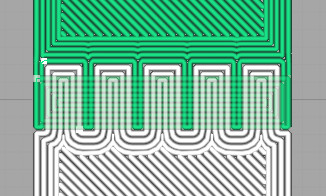
\includegraphics[width=\figheight,rotate=90]{sources/testing/straight_gcode.jpg}
		\caption{Straight}
		\label{fig:gcode_straight}
	\end{subfigure}
	\begin{subfigure}[B]{.26\columnwidth}
		\centering
		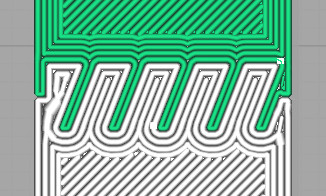
\includegraphics[width=\figheight,rotate=90]{sources/testing/diagonal_gcode.jpg}
		\caption{Diagonal}
		\label{fig:gcode_diagonal}
	\end{subfigure}
	\begin{subfigure}[B]{.22\columnwidth}
		\centering
		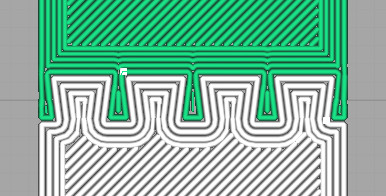
\includegraphics[width=\figheight,rotate=90]{sources/testing/suture_gcode.jpg}
		\caption{Trap. suture}
		\label{fig:gcode_suture}
	\end{subfigure}
	\begin{subfigure}[B]{.22\columnwidth}
		\centering
		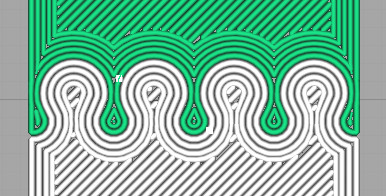
\includegraphics[width=\figheight,rotate=90]{sources/testing/jigsaw_gcode.jpg}
		\caption{Jigsaw}
		\label{fig:gcode_jigsaw}
	\end{subfigure}
	\caption{Gcodes generated with Cura Arachne engine beta. The layers of main fingers are shown and the other layers in a transparent overlay. While the straight and diagonal ITIM lattice produce continuous extrusion beads, the toolpaths for the dovetail designs include small separated segments.}
	\label{fig:gcode}
\end{figure}





\subsubsection{Model parameters}
\paragraph{Straight}
The straight design suffers from the curse of dimensionality;
even when setting $\wa=\SI{0.6}{\milli\meter}$, $\hc=\SI{0.1}{\milli\meter}$ and $L=\SI{3.6}{\milli\meter}$,
there are still the three free design variables $\wb$, $\va$ and $\hf$ to determine.
With 5 specimens per sample point and limited resources, the total number of data points we are able to test is limited.
We therefore chose to sample close to the two optima of the analytical models: whole and broken, as well as deviations from those optima in both directions along the axis of each design variable.
See \cref{fig:test_points_straight}.

Each sample of the straight orientation has $5\times5$ cells.
Because the repetition of cells is broken at the sides of the specimen, the boundary cells are adjusted for manufacturability and stability.
The specimens end with a TPLA finger on both sides and in cross beams on both top and bottom.
See \cref{fig:test_straight_boundary_cells}.

\begin{figure}
	\centering
	\begin{subfigure}[B]{.24\columnwidth}
		\centering
		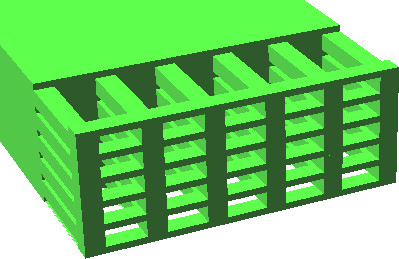
\includegraphics[width=\columnwidth]{sources/testing/straight_sample.jpg}
		\caption{Example print mesh near optimum}
		\label{fig:test_straight_boundary_cells}
	\end{subfigure}
	\begin{subfigure}[B]{.24\columnwidth}
		\centering
		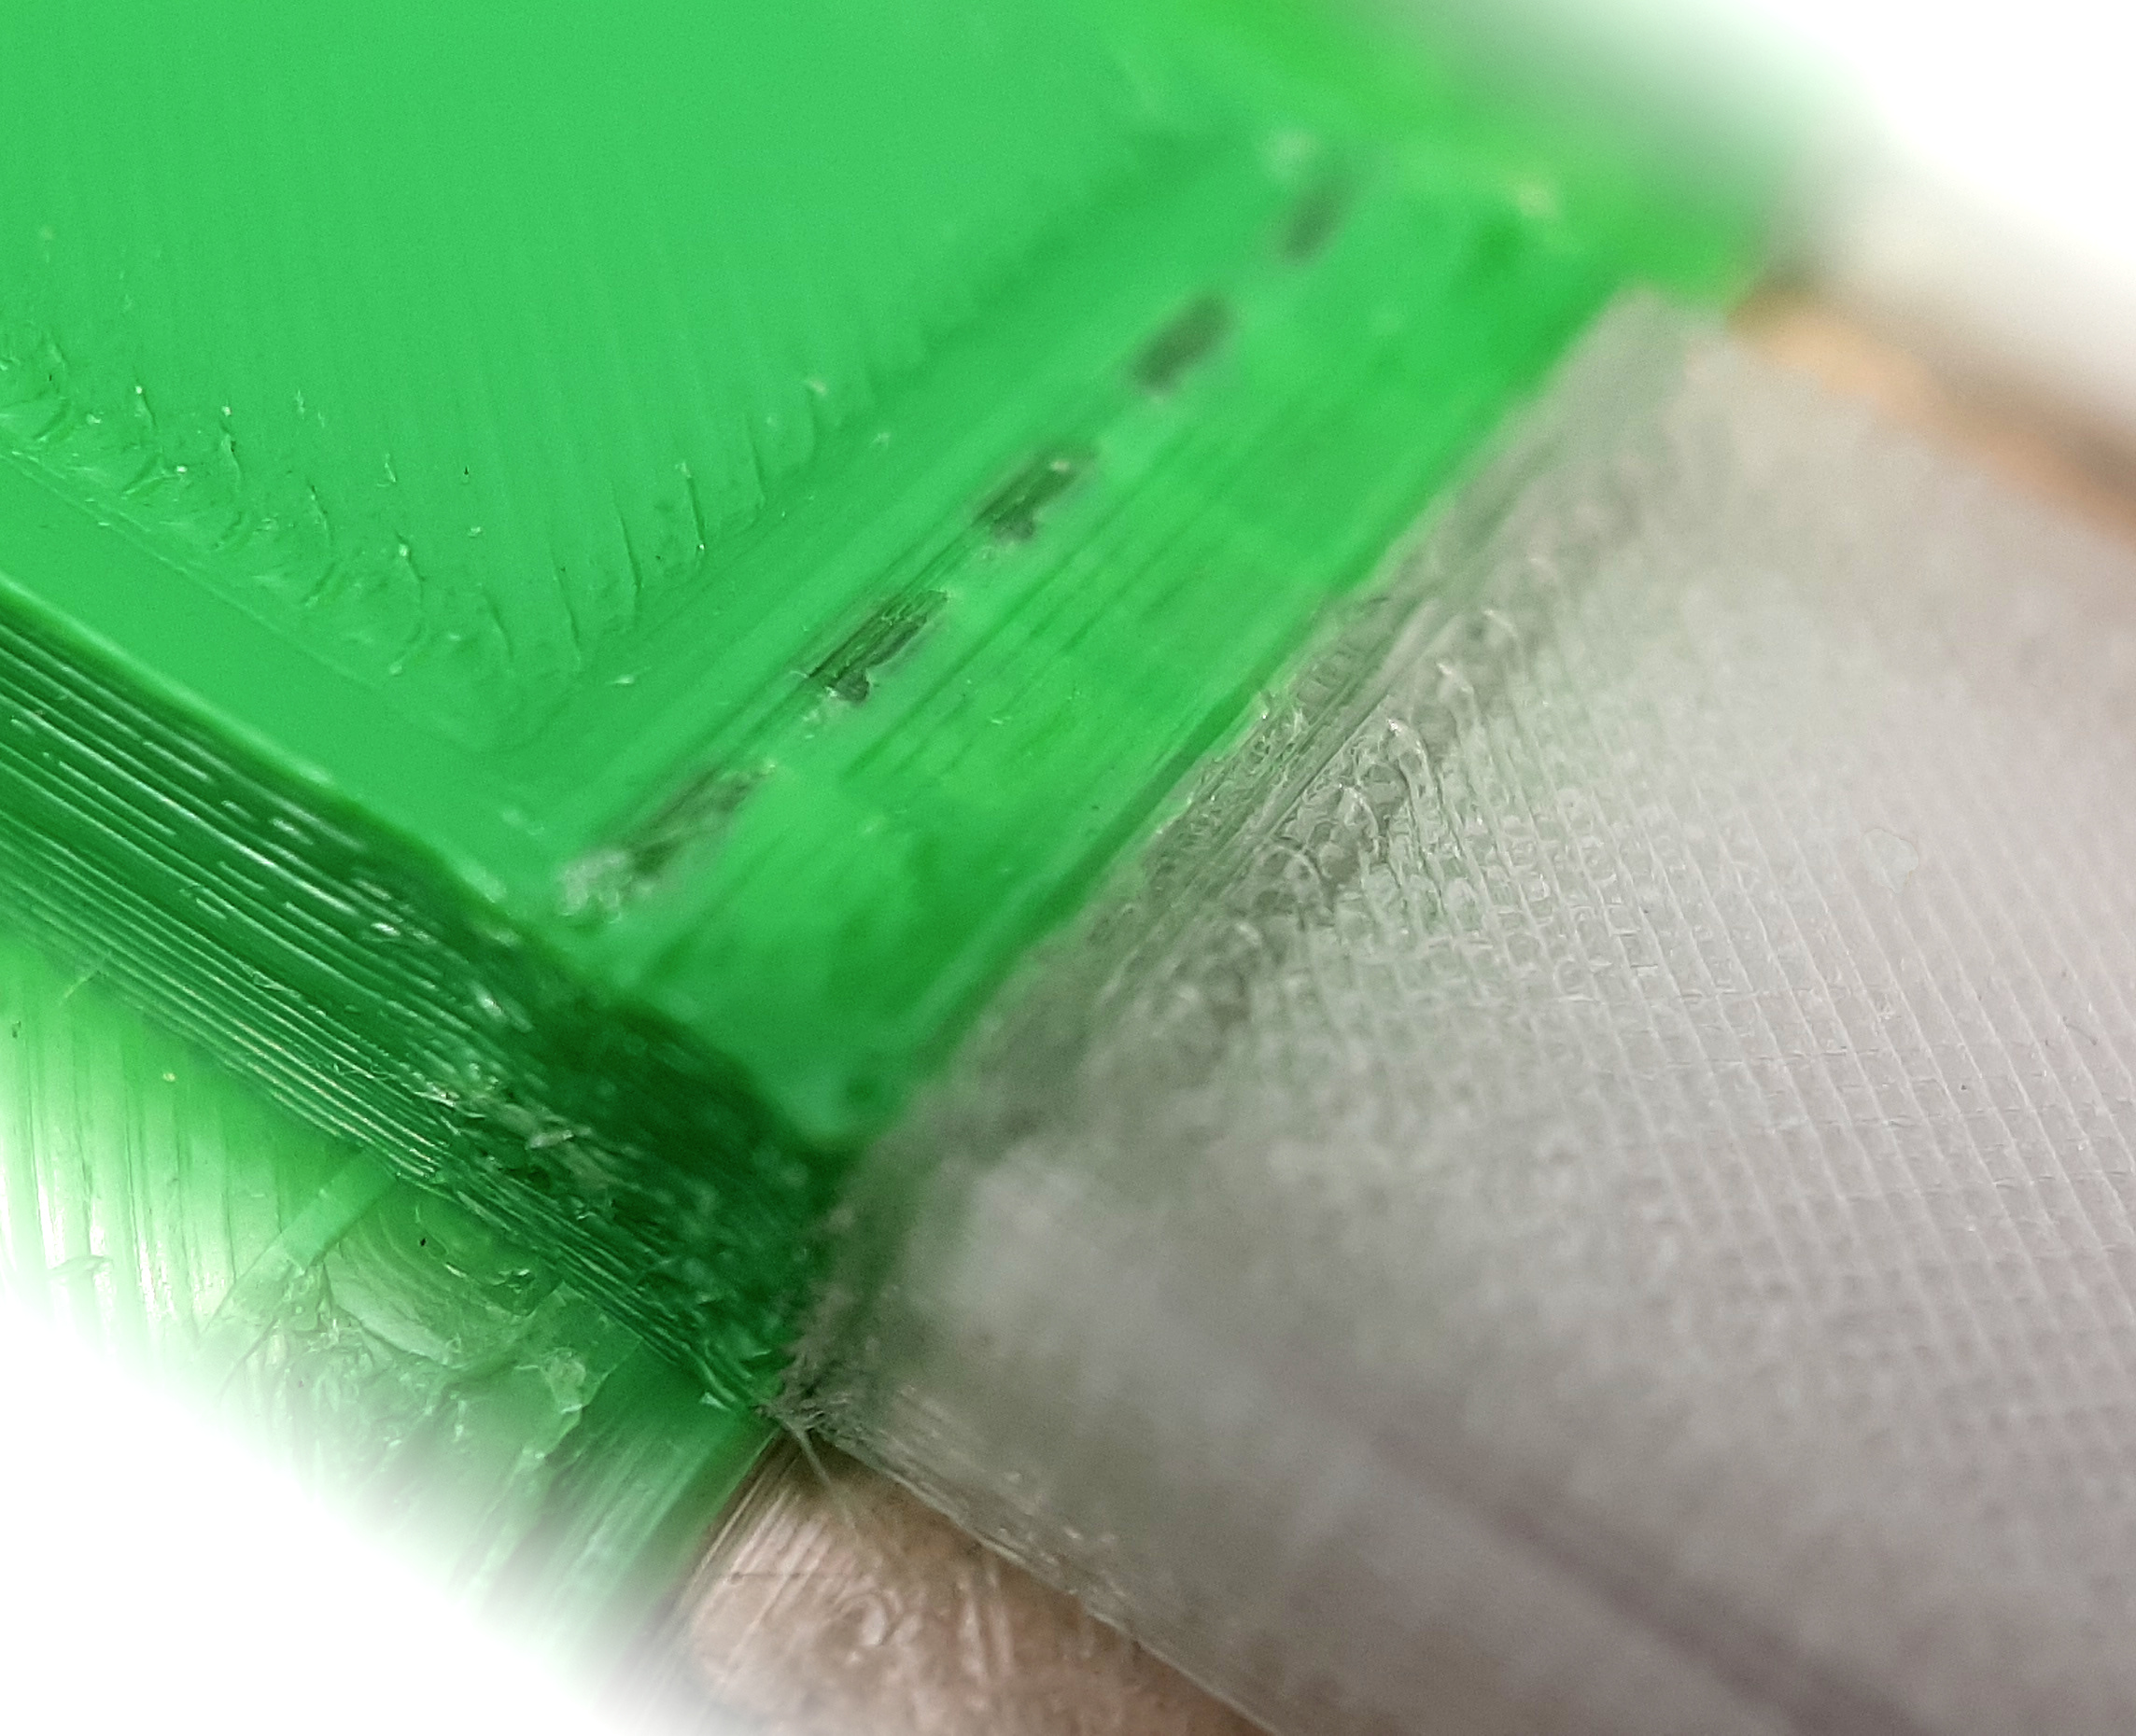
\includegraphics[width=\columnwidth]{sources/testing/straight_print.jpg}
		\caption{Example print near broken optimum}
	\end{subfigure}
	\begin{subfigure}[B]{.5\columnwidth}
		\centering
		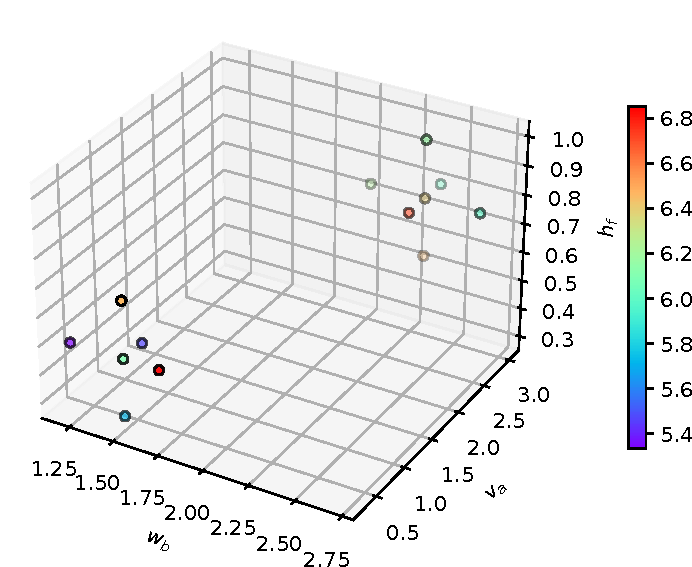
\includegraphics[width=\columnwidth]{sources/testing/straight_sample_points.pdf}
		\caption{Sampled points and measured cell stress}
		\label{fig:test_points_straight}
	\end{subfigure}
	\caption{Experimental setup of straight design.}
\end{figure}





\paragraph{Diagonal}
Each sample of the diagonal orientation contains 5 cells in the horizontal direction, but 13 repetition in Z because of the low unit cell height.
Extra finger beams are added to the sides of the specimen to prevent any part of the beam to be less than $2\wmin=\SI{0.6}{\milli\meter}$ wide.
See \cref{fig:gcode_diagonal}.
Because with a given $L=\SI{3.6}{\milli\meter}$, $h=\SI{0.2}{\milli\meter}$ and $\wa=\SI{0.6}{\milli\meter}$ the remaining design space is only one-dimensional,
we can simply sample various points along $\wb$: $(0.6, 1.2, 1.8, 2.4, 3.0, 3.6)$.

\iffalse
\begin{figure}
	\centering
	\begin{subfigure}[B]{.24\columnwidth}
		\centering
		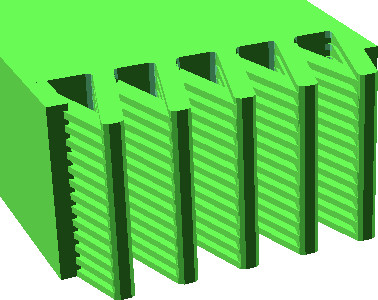
\includegraphics[width=\columnwidth]{sources/testing/diagonal_sample.jpg}
		\caption{Example print mesh}
		\label{fig:test_diagonal_boundary_cells}
	\end{subfigure}
	\begin{subfigure}[B]{.24\columnwidth}
		\centering
		\includegraphics[width=\columnwidth]{sources/testing/diagonal_print.jpg}
		\caption{Example print}
	\end{subfigure}
	\begin{subfigure}[B]{.5\columnwidth}
		\centering
		%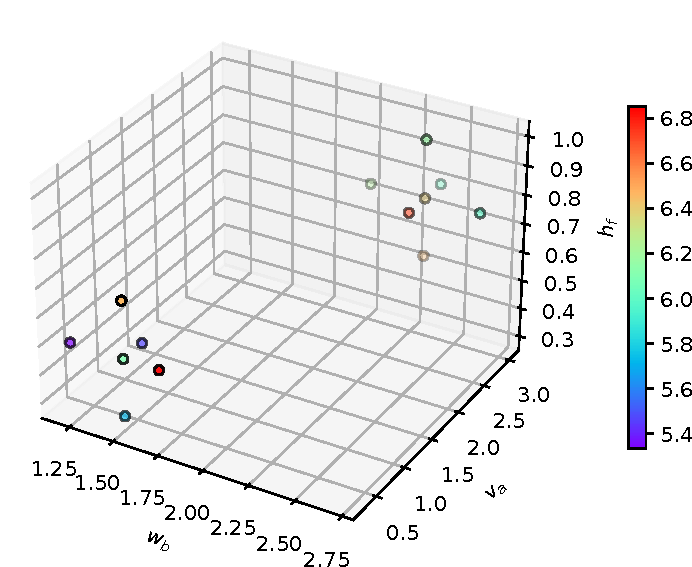
\includegraphics[width=\columnwidth]{sources/testing/straight_sample_points.pdf}
		\caption{Comparison of results to analytical model}
	\end{subfigure}
	\caption{Experimental setup of diagonal design.}
\end{figure}
\fi







\begin{figure}
	\centering
	\begin{subfigure}{.49\columnwidth}
		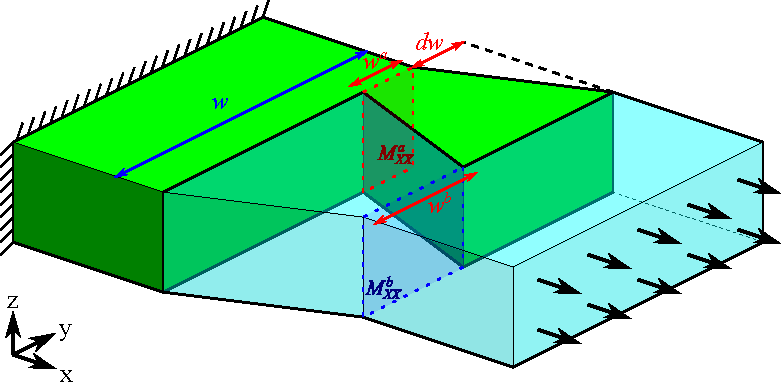
\includegraphics{sources/method/suture_model_v5.pdf}
		\caption{Trapezoidal suture}
		\label{fig:suture}
	\end{subfigure}
	\begin{subfigure}{.49\columnwidth}
		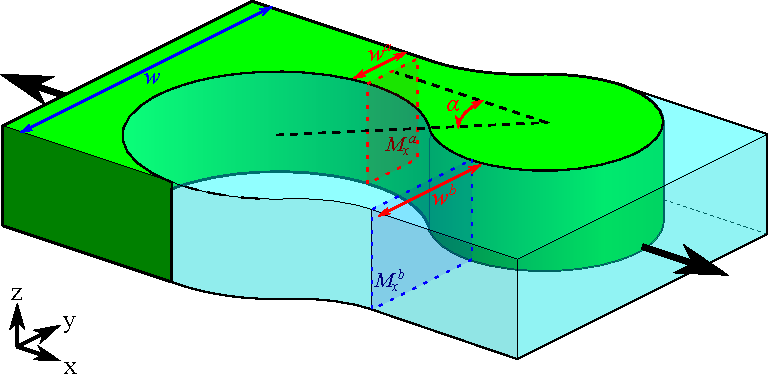
\includegraphics{sources/method/jigsaw_model_v5.pdf}
		\caption{Jigsaw}
		\label{fig:jigsaw}
	\end{subfigure}
	\caption{Simple 2D dovetail interlocking microstructures.}
	\label{fig:suture_jigsaw}
\end{figure}


\paragraph{Dovetail interlocking}
We compared our interlocking structures against two interlocking designs: trapezoidal sutures and jigsaw interlocking.
See \cref{fig:suture_jigsaw}.
We used $\wa=2\wmin{a}$, $dw=\SI{0.3}{\milli\meter}$ and $L=2.4$ for the trapezoidal suture,
and $\wa=2\wmin{a}$ and $\alpha = \SI{35}{\degree}$ for the jigsaw interlocking design.
We printed samples with both $\wb=3\wa$ and $\wb=\nicefrac{\sigmafail{a}}{\sigmafail{b}}\wa = 4.48 \wa$.
%The latter value is optimized for tensile failure along $\myz{b}$. >> not true!!!
We used 6 and 4 repetition respectively and a height of \SI{5}{\milli\meter}.

Note that the jigsaw interlocking structure is quite similar to the trapezoidal suture, with the addition of semicircles to the ends of the trapezoids.
The total length $L$ of the jigsaw structure is \SI{2.96}{\milli\meter} and \SI{4.05}{\milli\meter} for the two $\wb$ values respectively,
so the $\lmax$ constraint is violated by that structure.

The boundaries of these two structures end in half a TPLA lobe, because that is the stiffer material.
In order to meet the minimum width constraint there, the sides of the specimen are extruded by $\wmin{a}$; see \cref{fig:gcode_suture,fig:gcode_jigsaw}



\begin{figure*}
	\centering
	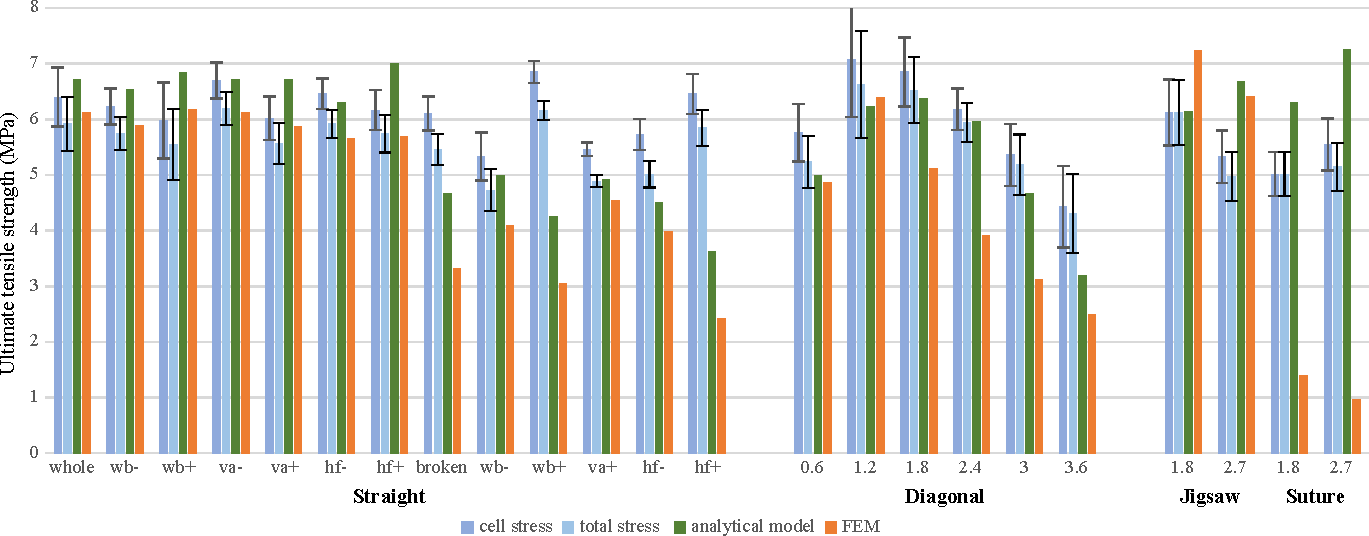
\includegraphics[width=\textwidth]{sources/testing/results.pdf}
	\caption{Test results compared to the predictions according to the analytical model and the RBF network fitted to the simulation results. The straight model samples are labelled relative to the whole and broken optimum, while the rest is labelled by their $\wb$ value.}
	\label{fig:test_results}
\end{figure*}


\subsubsection{Results}
After tensile testing we can observe various failure modes, such as in \cref{fig:failures}.
The tensile tests performed result in force-displacement graphs such as displayed in \cref{fig:stress_displacement_comparison},
from which the ultimate tensile strength values are derived.
Because the boundary cells deviate from the regular pattern, computing the ultimate tensile strength can be done in two ways, giving rise to two statistics.
We compute the \emph{cell stress} by dividing the maximum force of the force-displacement graphs by the number of cells and then divide it by the cross sectional area of the cell.
We compute the \emph{total stress} by dividing the force by the total cross-sectional area of the sample, including the extra geometry at the boundaries of the sample.
Ideally we would compensate for manufacturing inaccuracies by using measured dimensions of the specimens,
but measuring the internal geometry of the interlocking structure is practically infeasible, so we use the dimensions of the 3D mesh instead.
The results from the physical experiments, along with the analytical and simulated predictions are gathered in \cref{fig:test_results}.


\begin{figure}
	\centering
	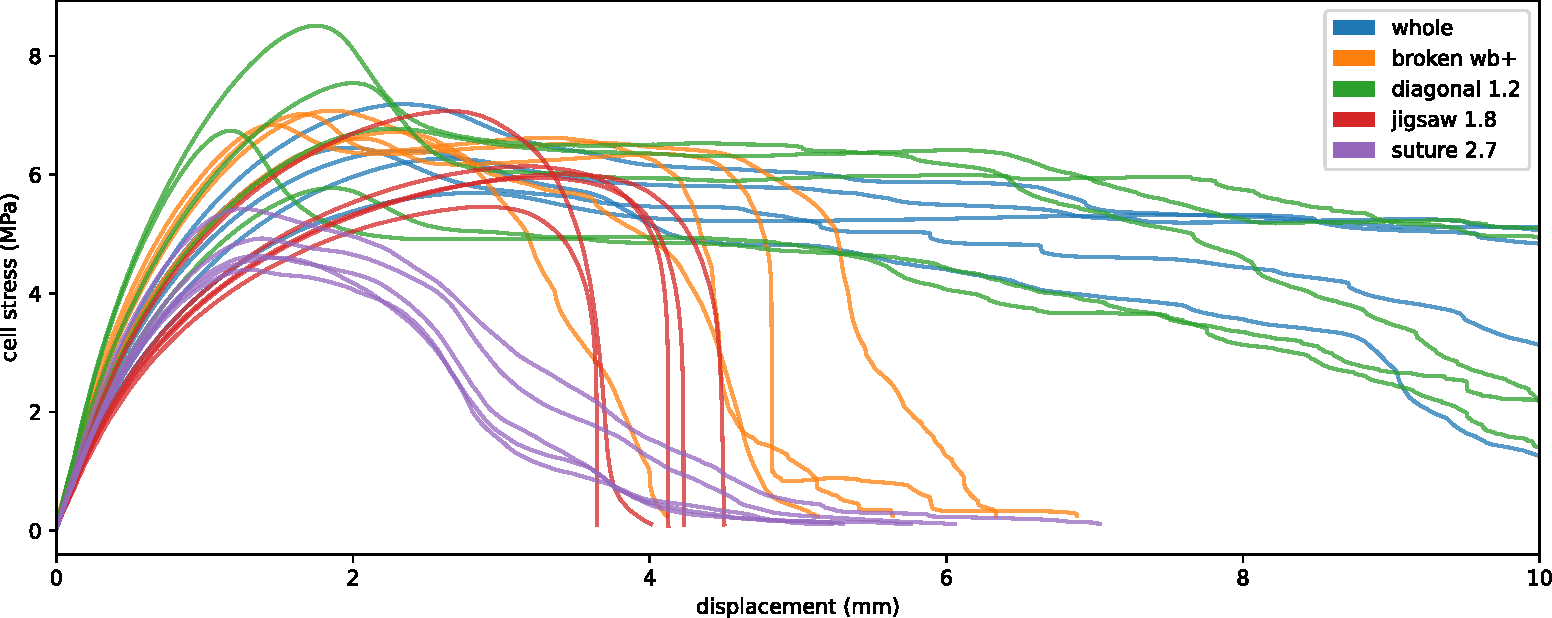
\includegraphics[width=\columnwidth]{sources/testing/stress_displacement_comparison.pdf}
	\caption{Comparison of the best performing design of each type. 
		The diagonal design with $\wb=\SI{1.2}{\milli\meter}$ showed the highest maximum tensile stress. 
		By inspecting the shape of the graph you can determine the dominant failure mode: TPLA breaking (sharp drop) or PP yielding (plateau).
		Dovetail unlocking has either a sharp drop or a more gradual decline.
	}
	\label{fig:stress_displacement_comparison}
\end{figure}



\begin{figure}
	\setlength{\figwidth}{.19\columnwidth}
	\begin{subfigure}[B]{.99\columnwidth}
		\centering
		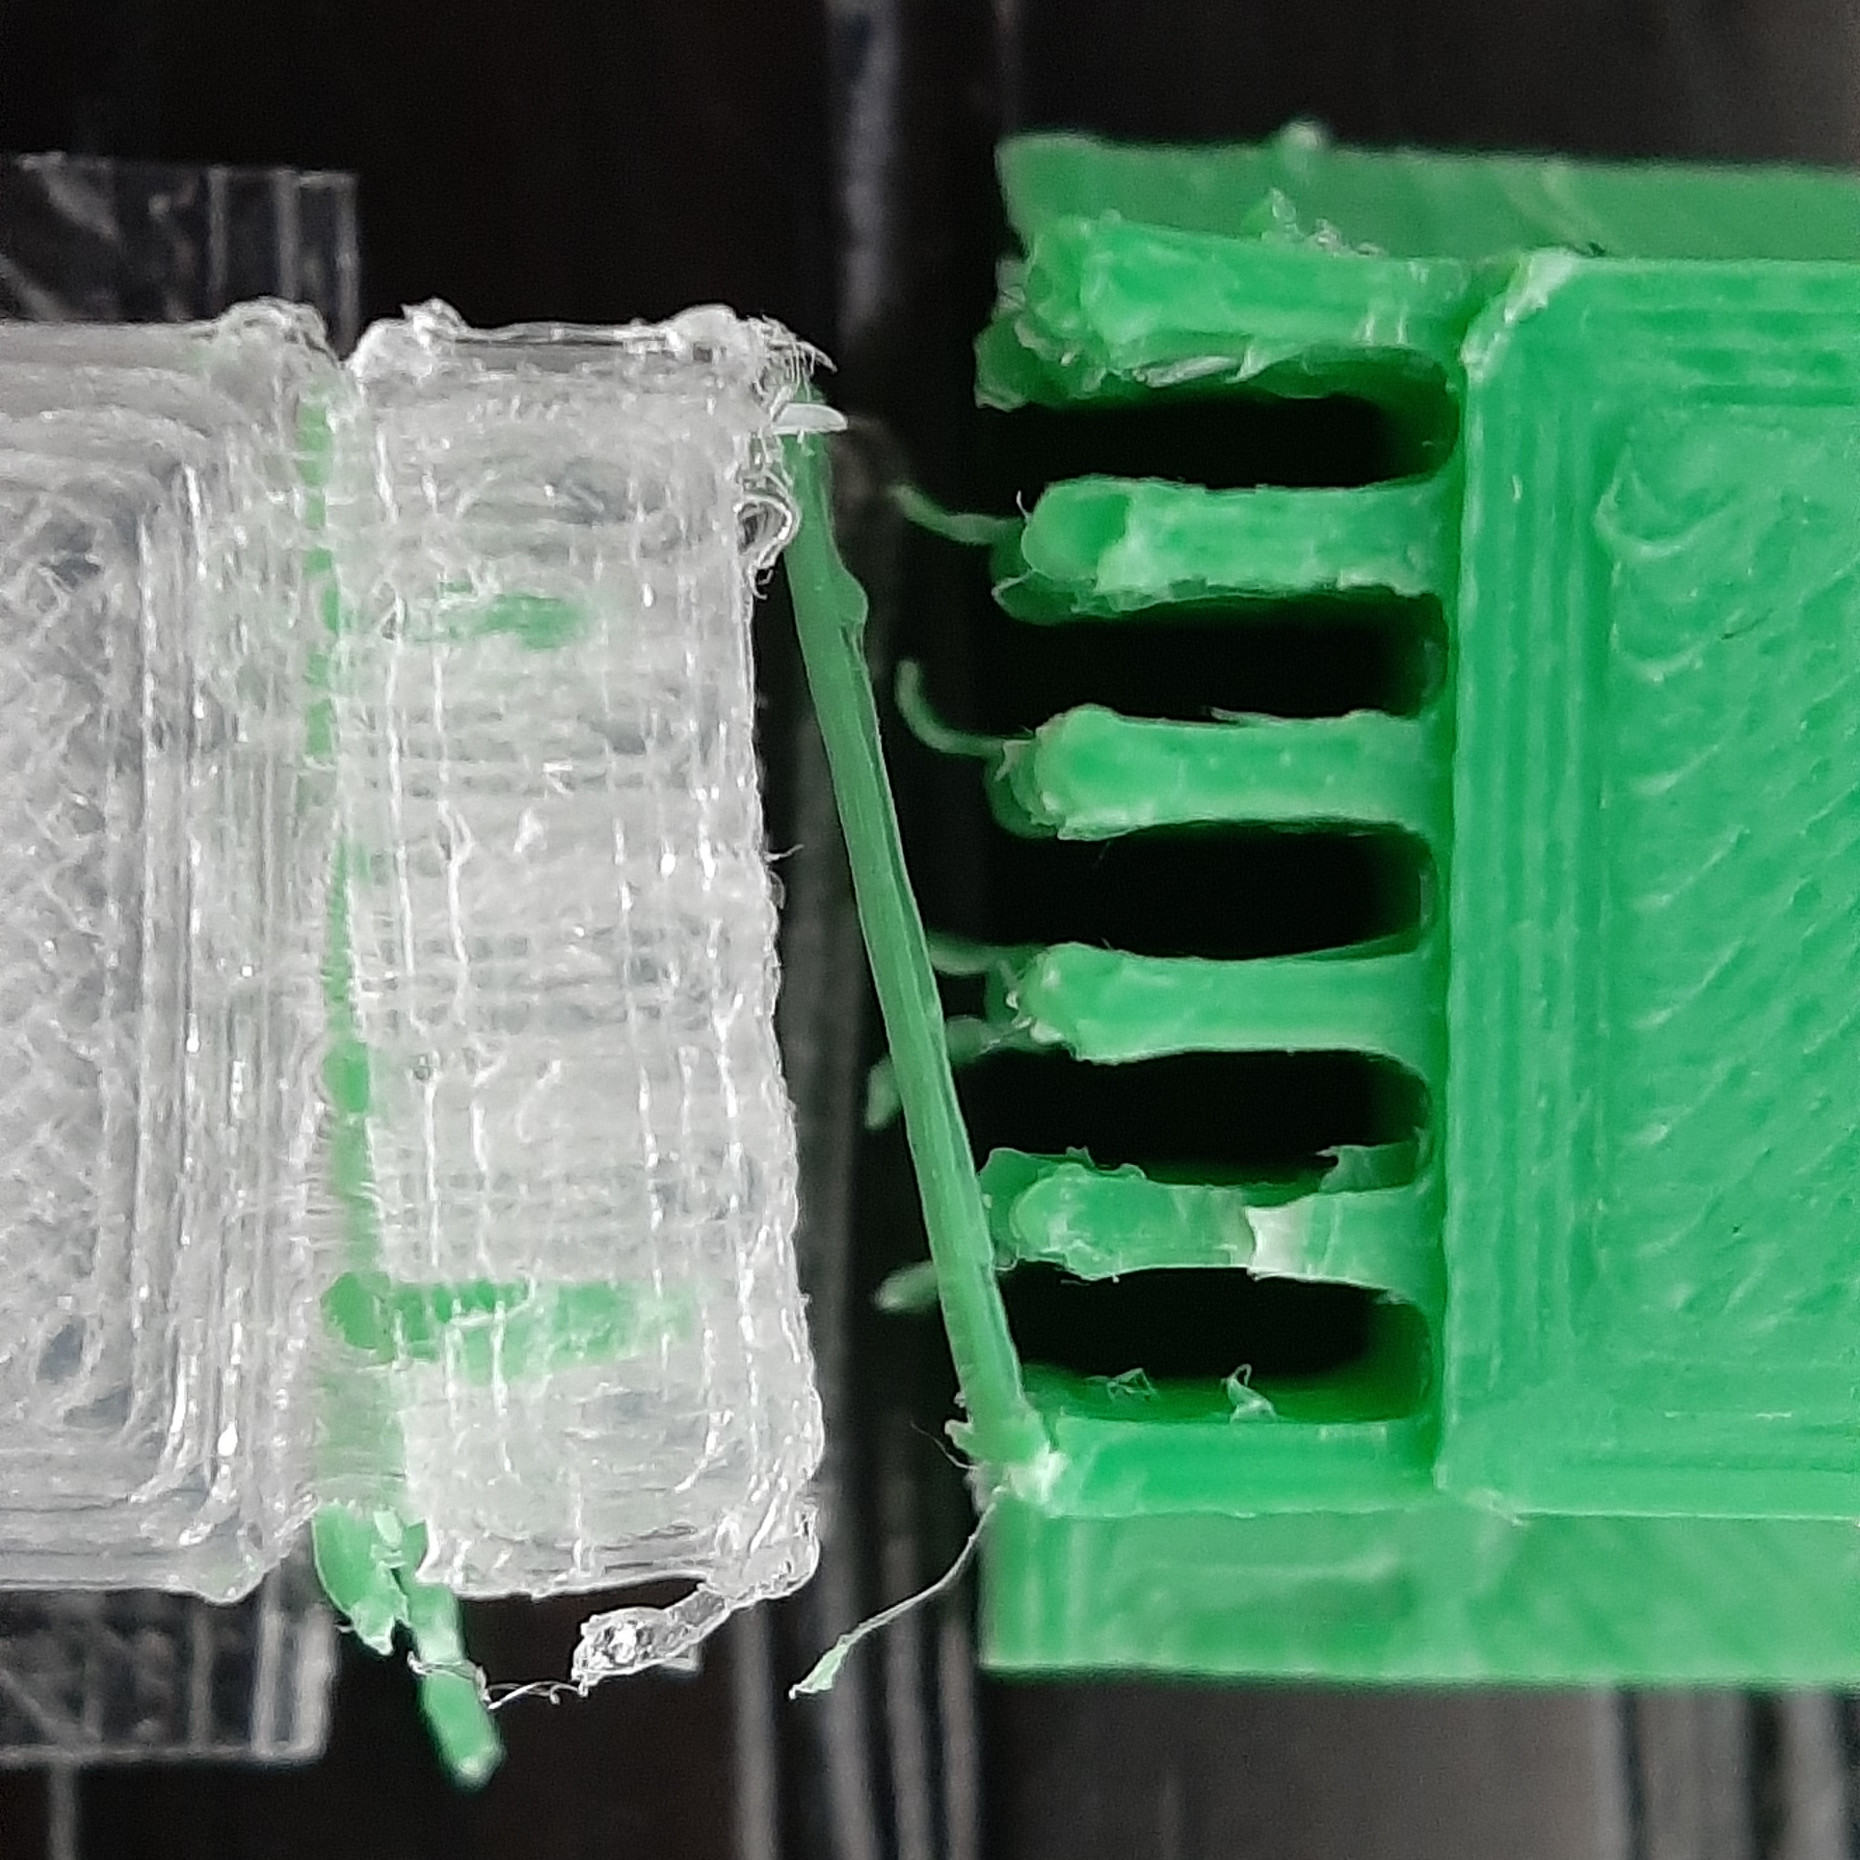
\includegraphics[width=\figwidth]{sources/testing/j1_cropped.jpg}
		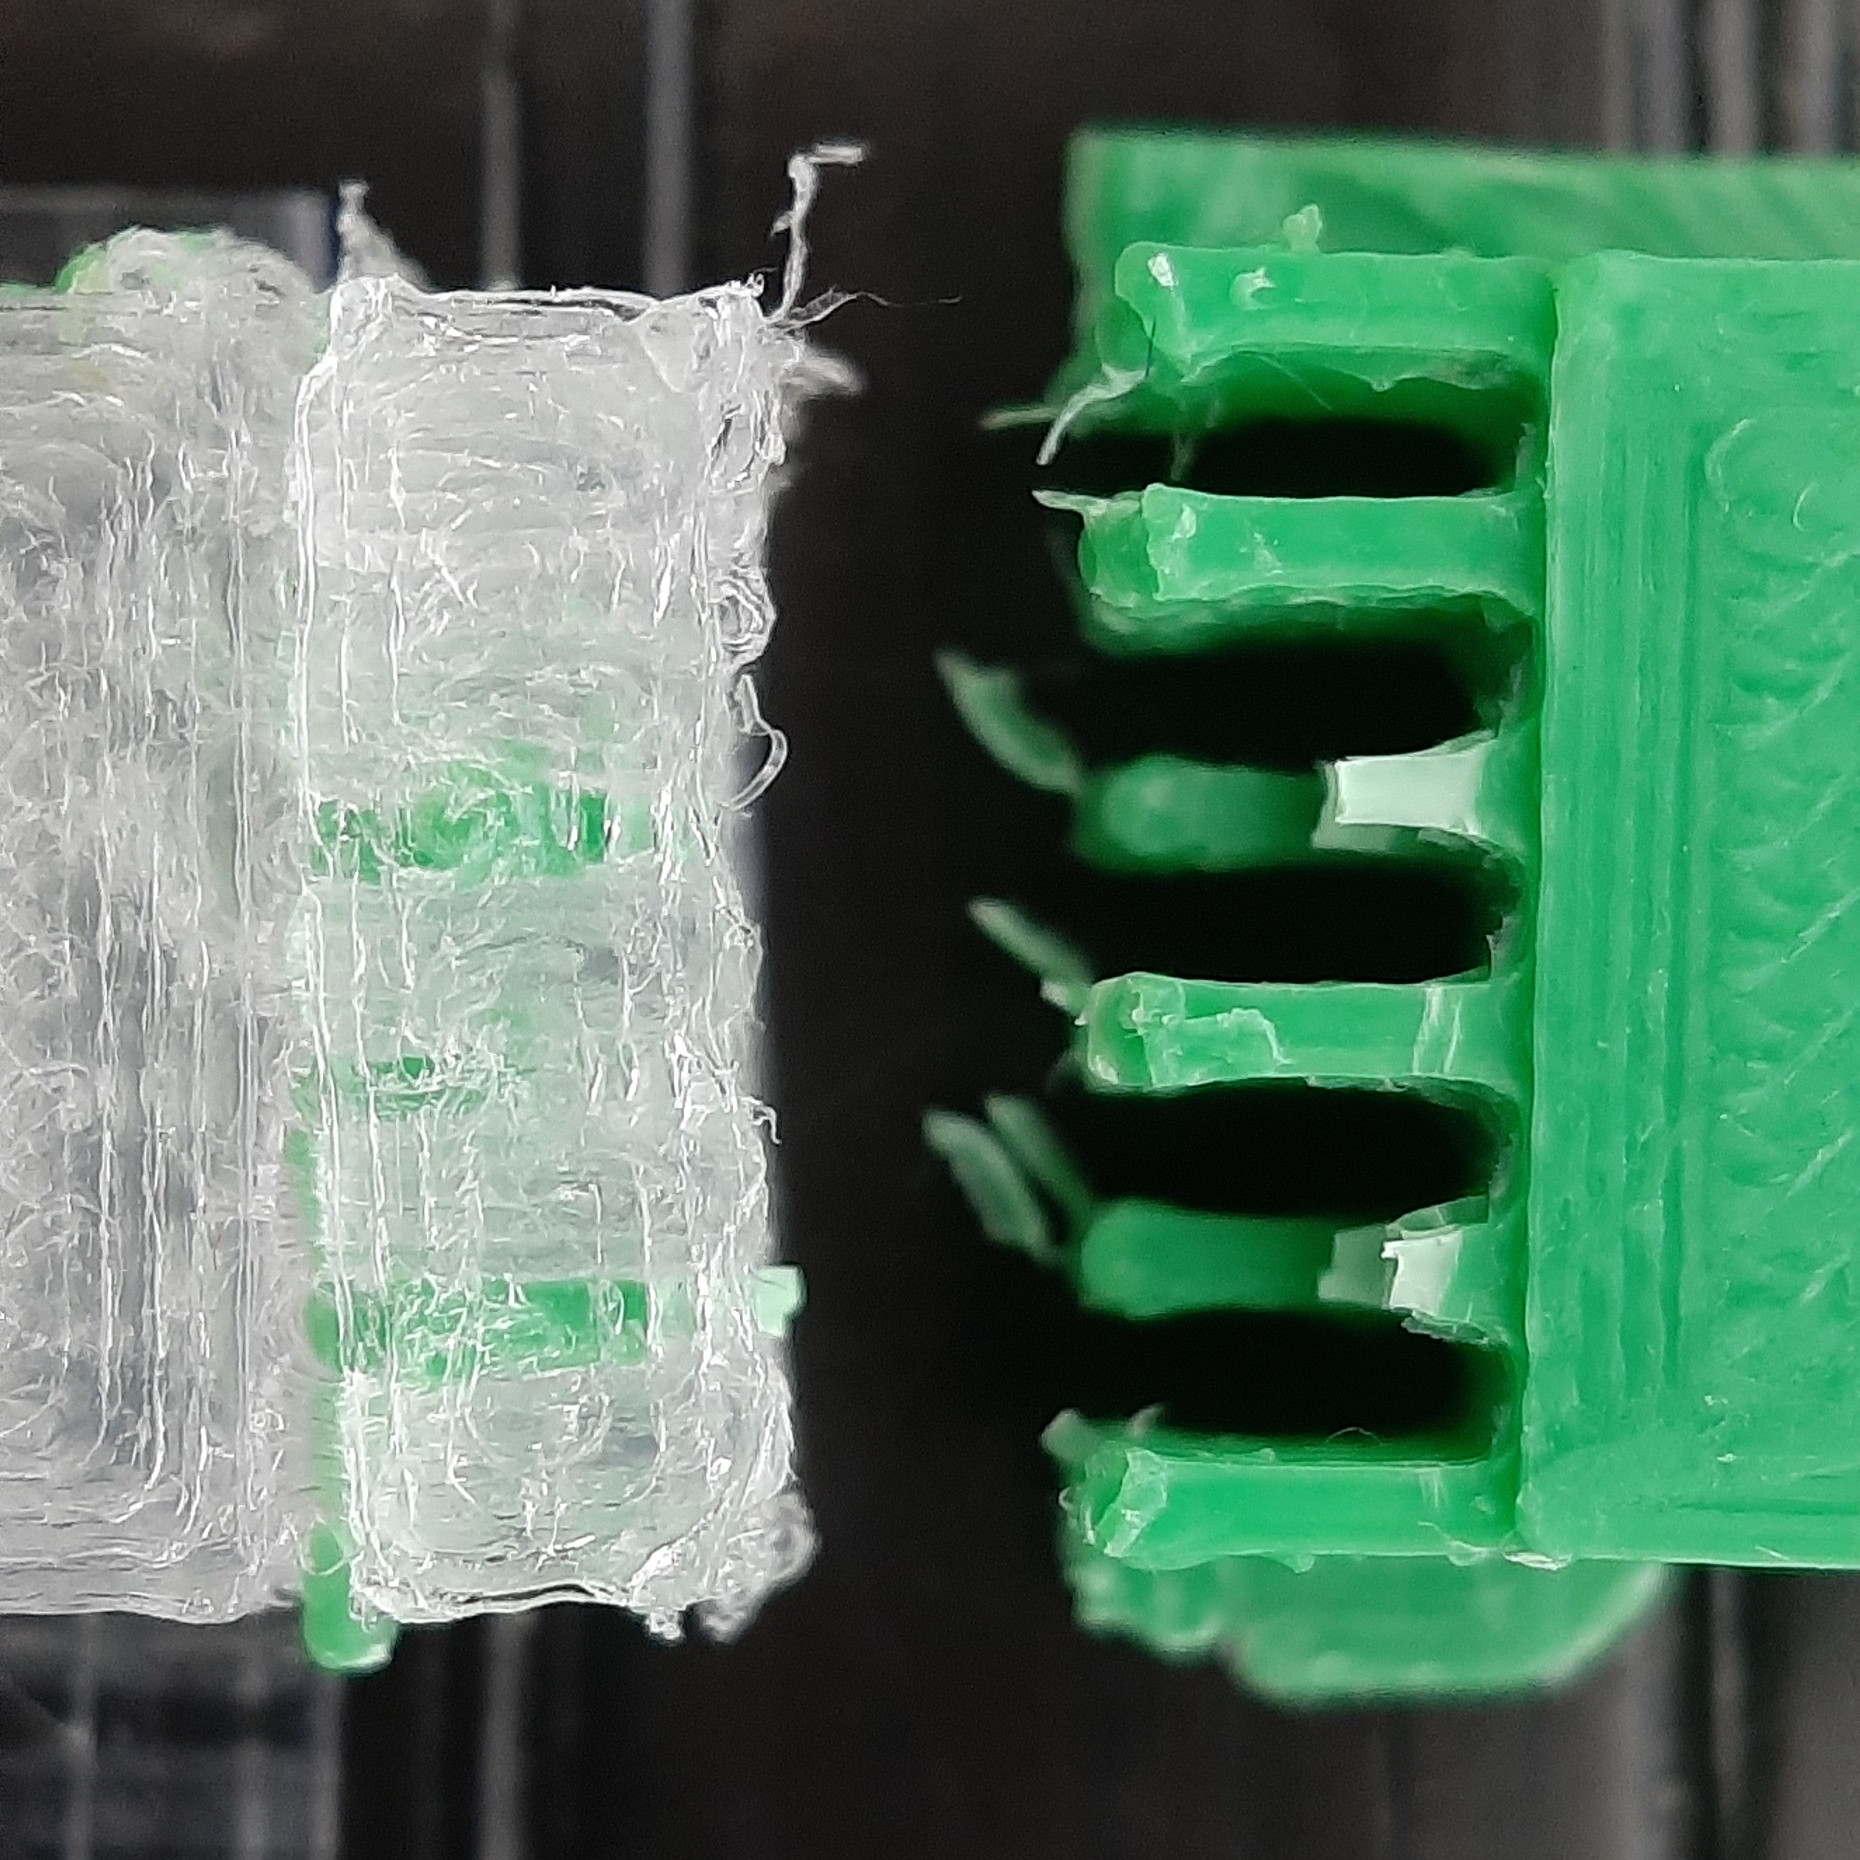
\includegraphics[width=\figwidth]{sources/testing/j2_cropped.jpg}
		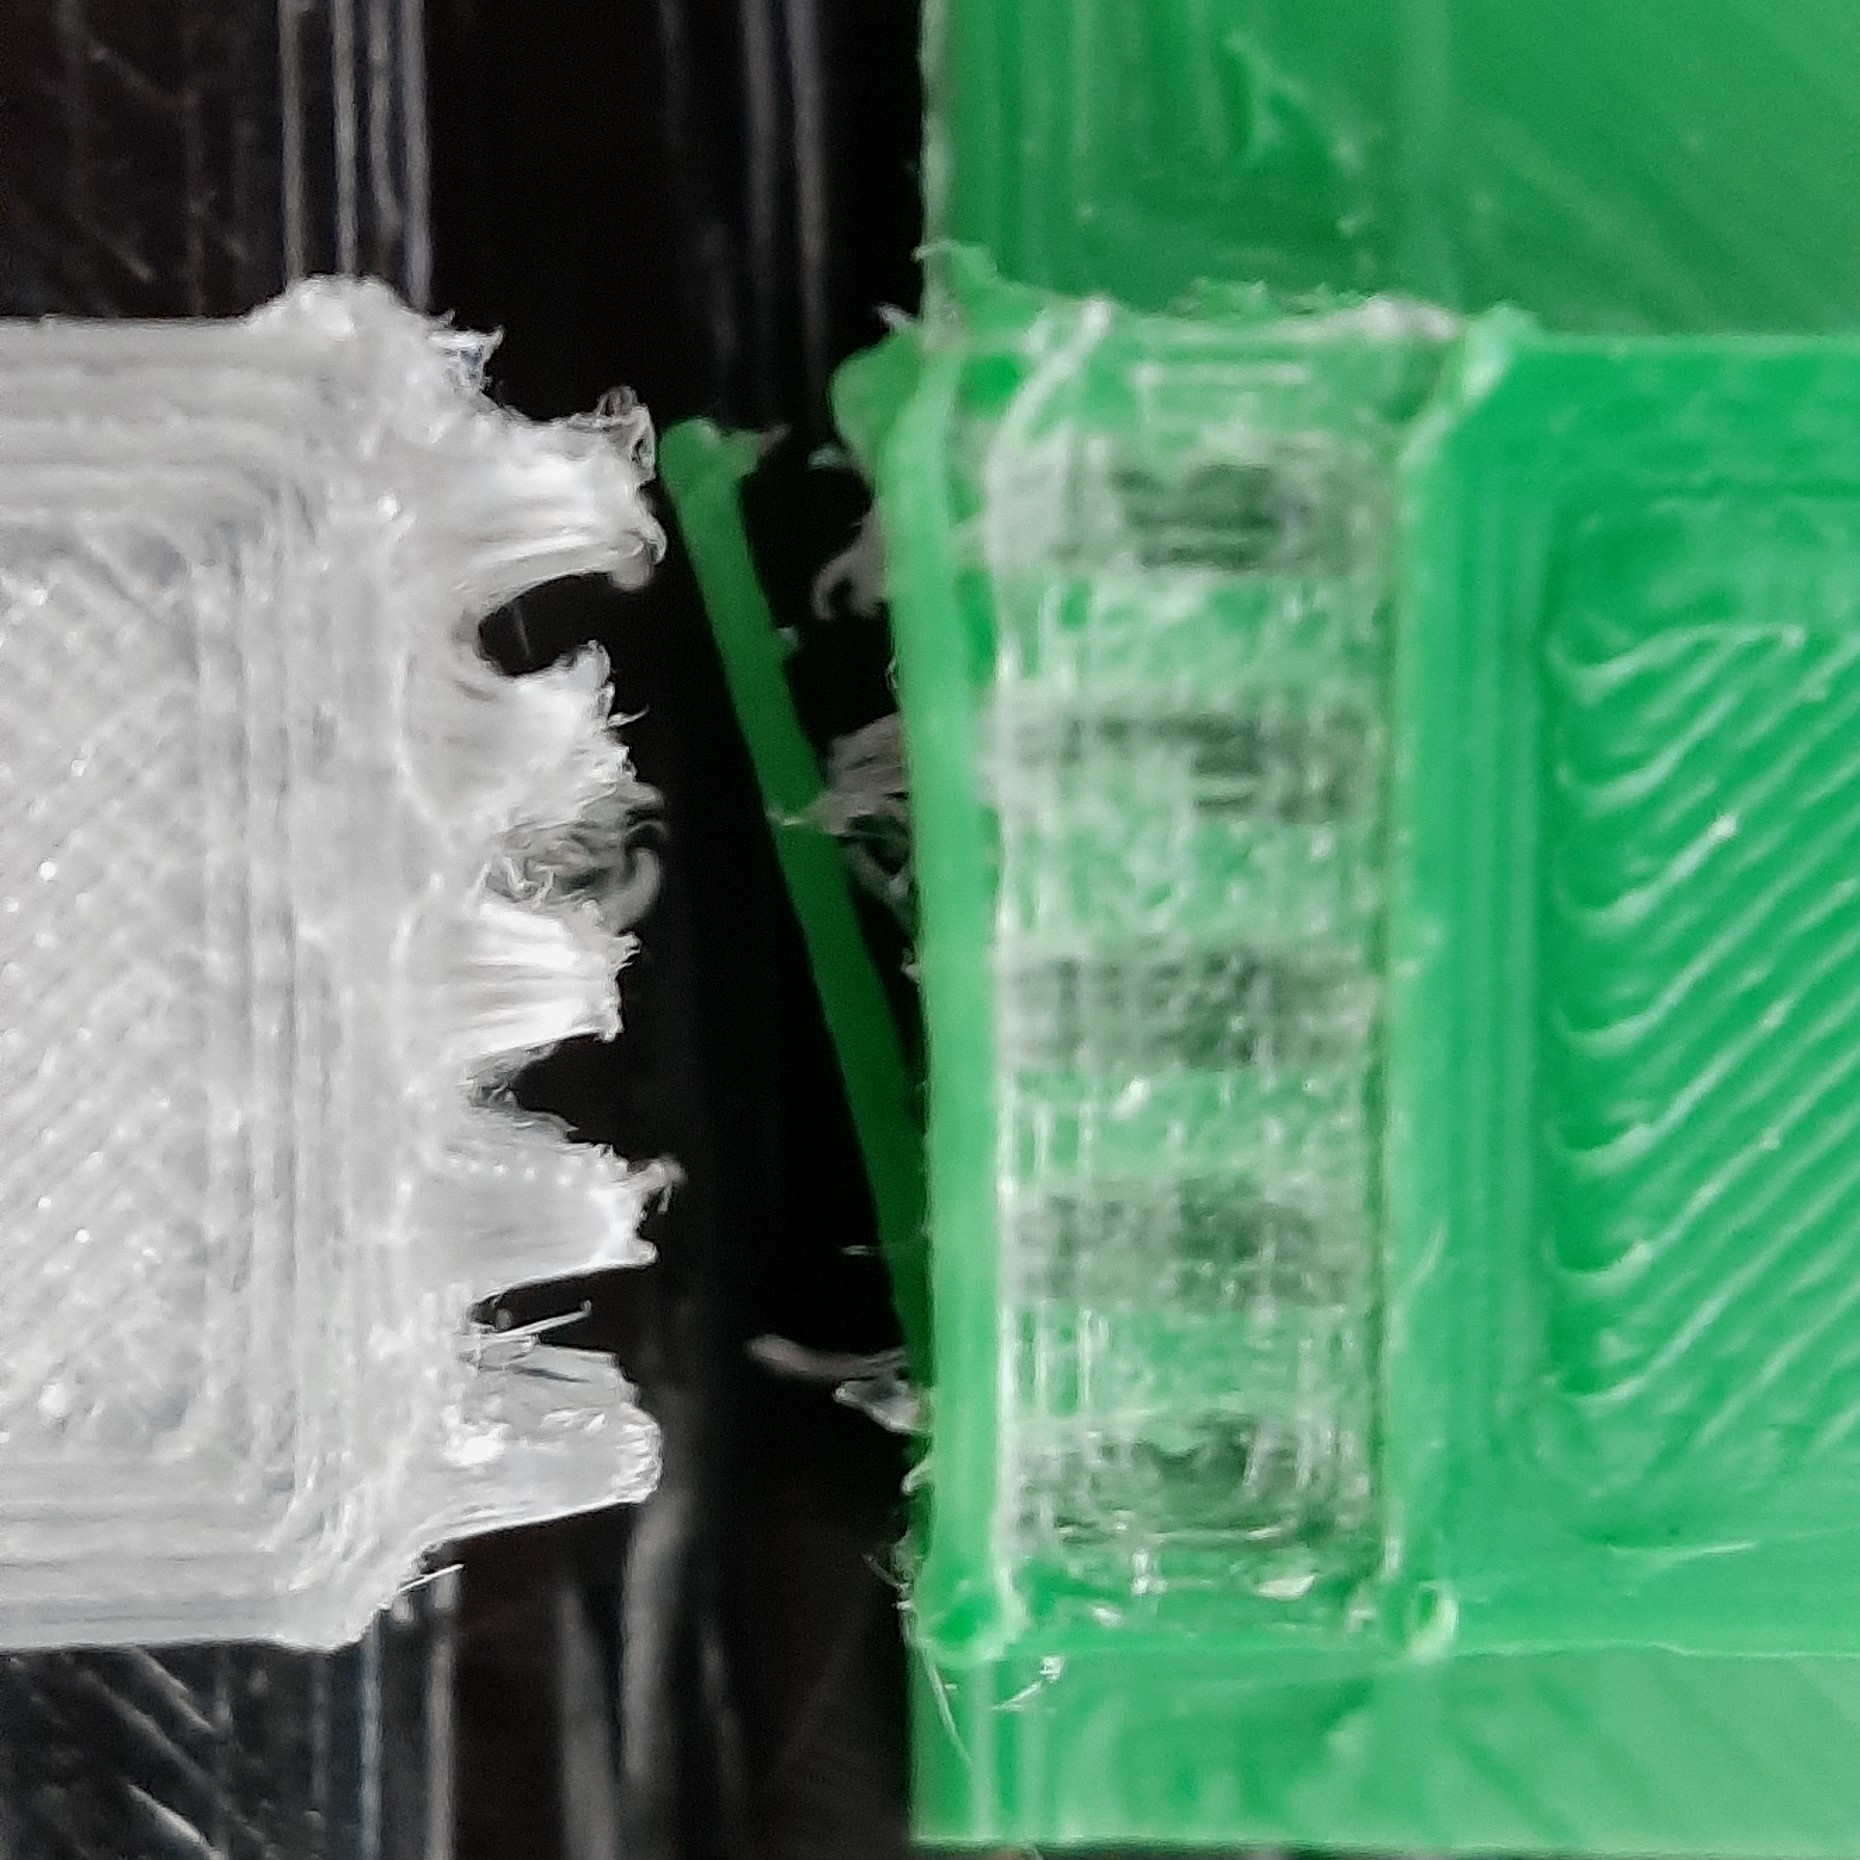
\includegraphics[width=\figwidth]{sources/testing/j3_cropped.jpg}
		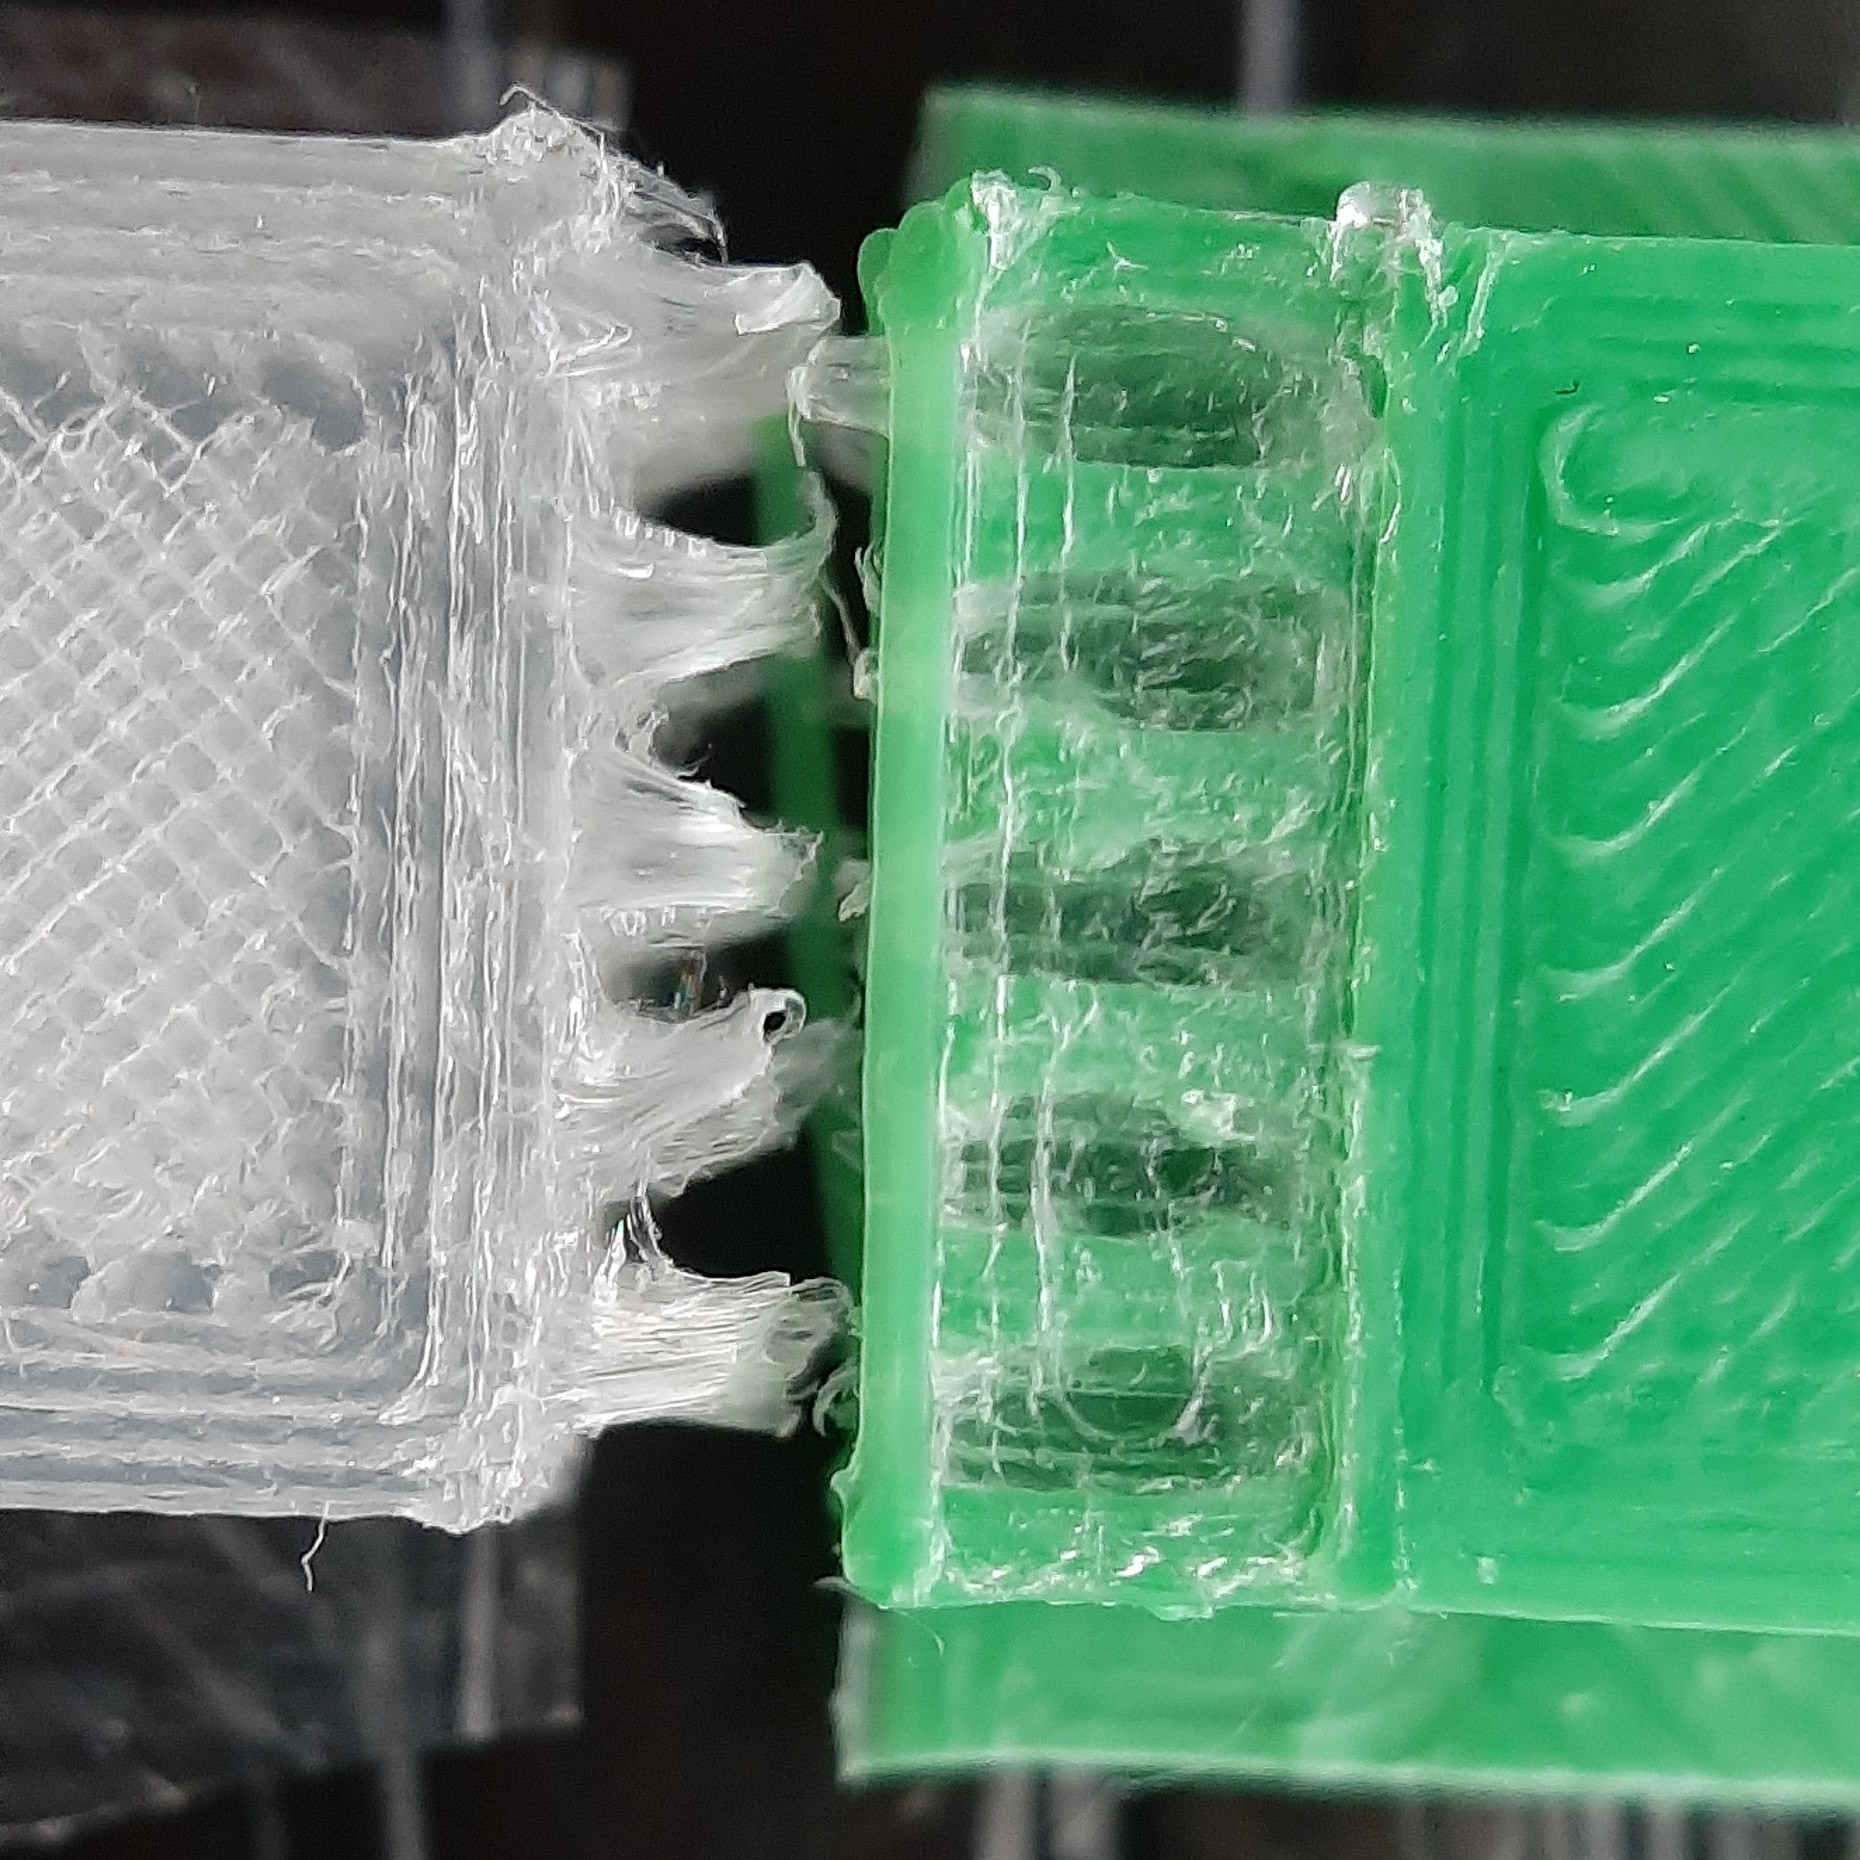
\includegraphics[width=\figwidth]{sources/testing/j4_cropped.jpg}
		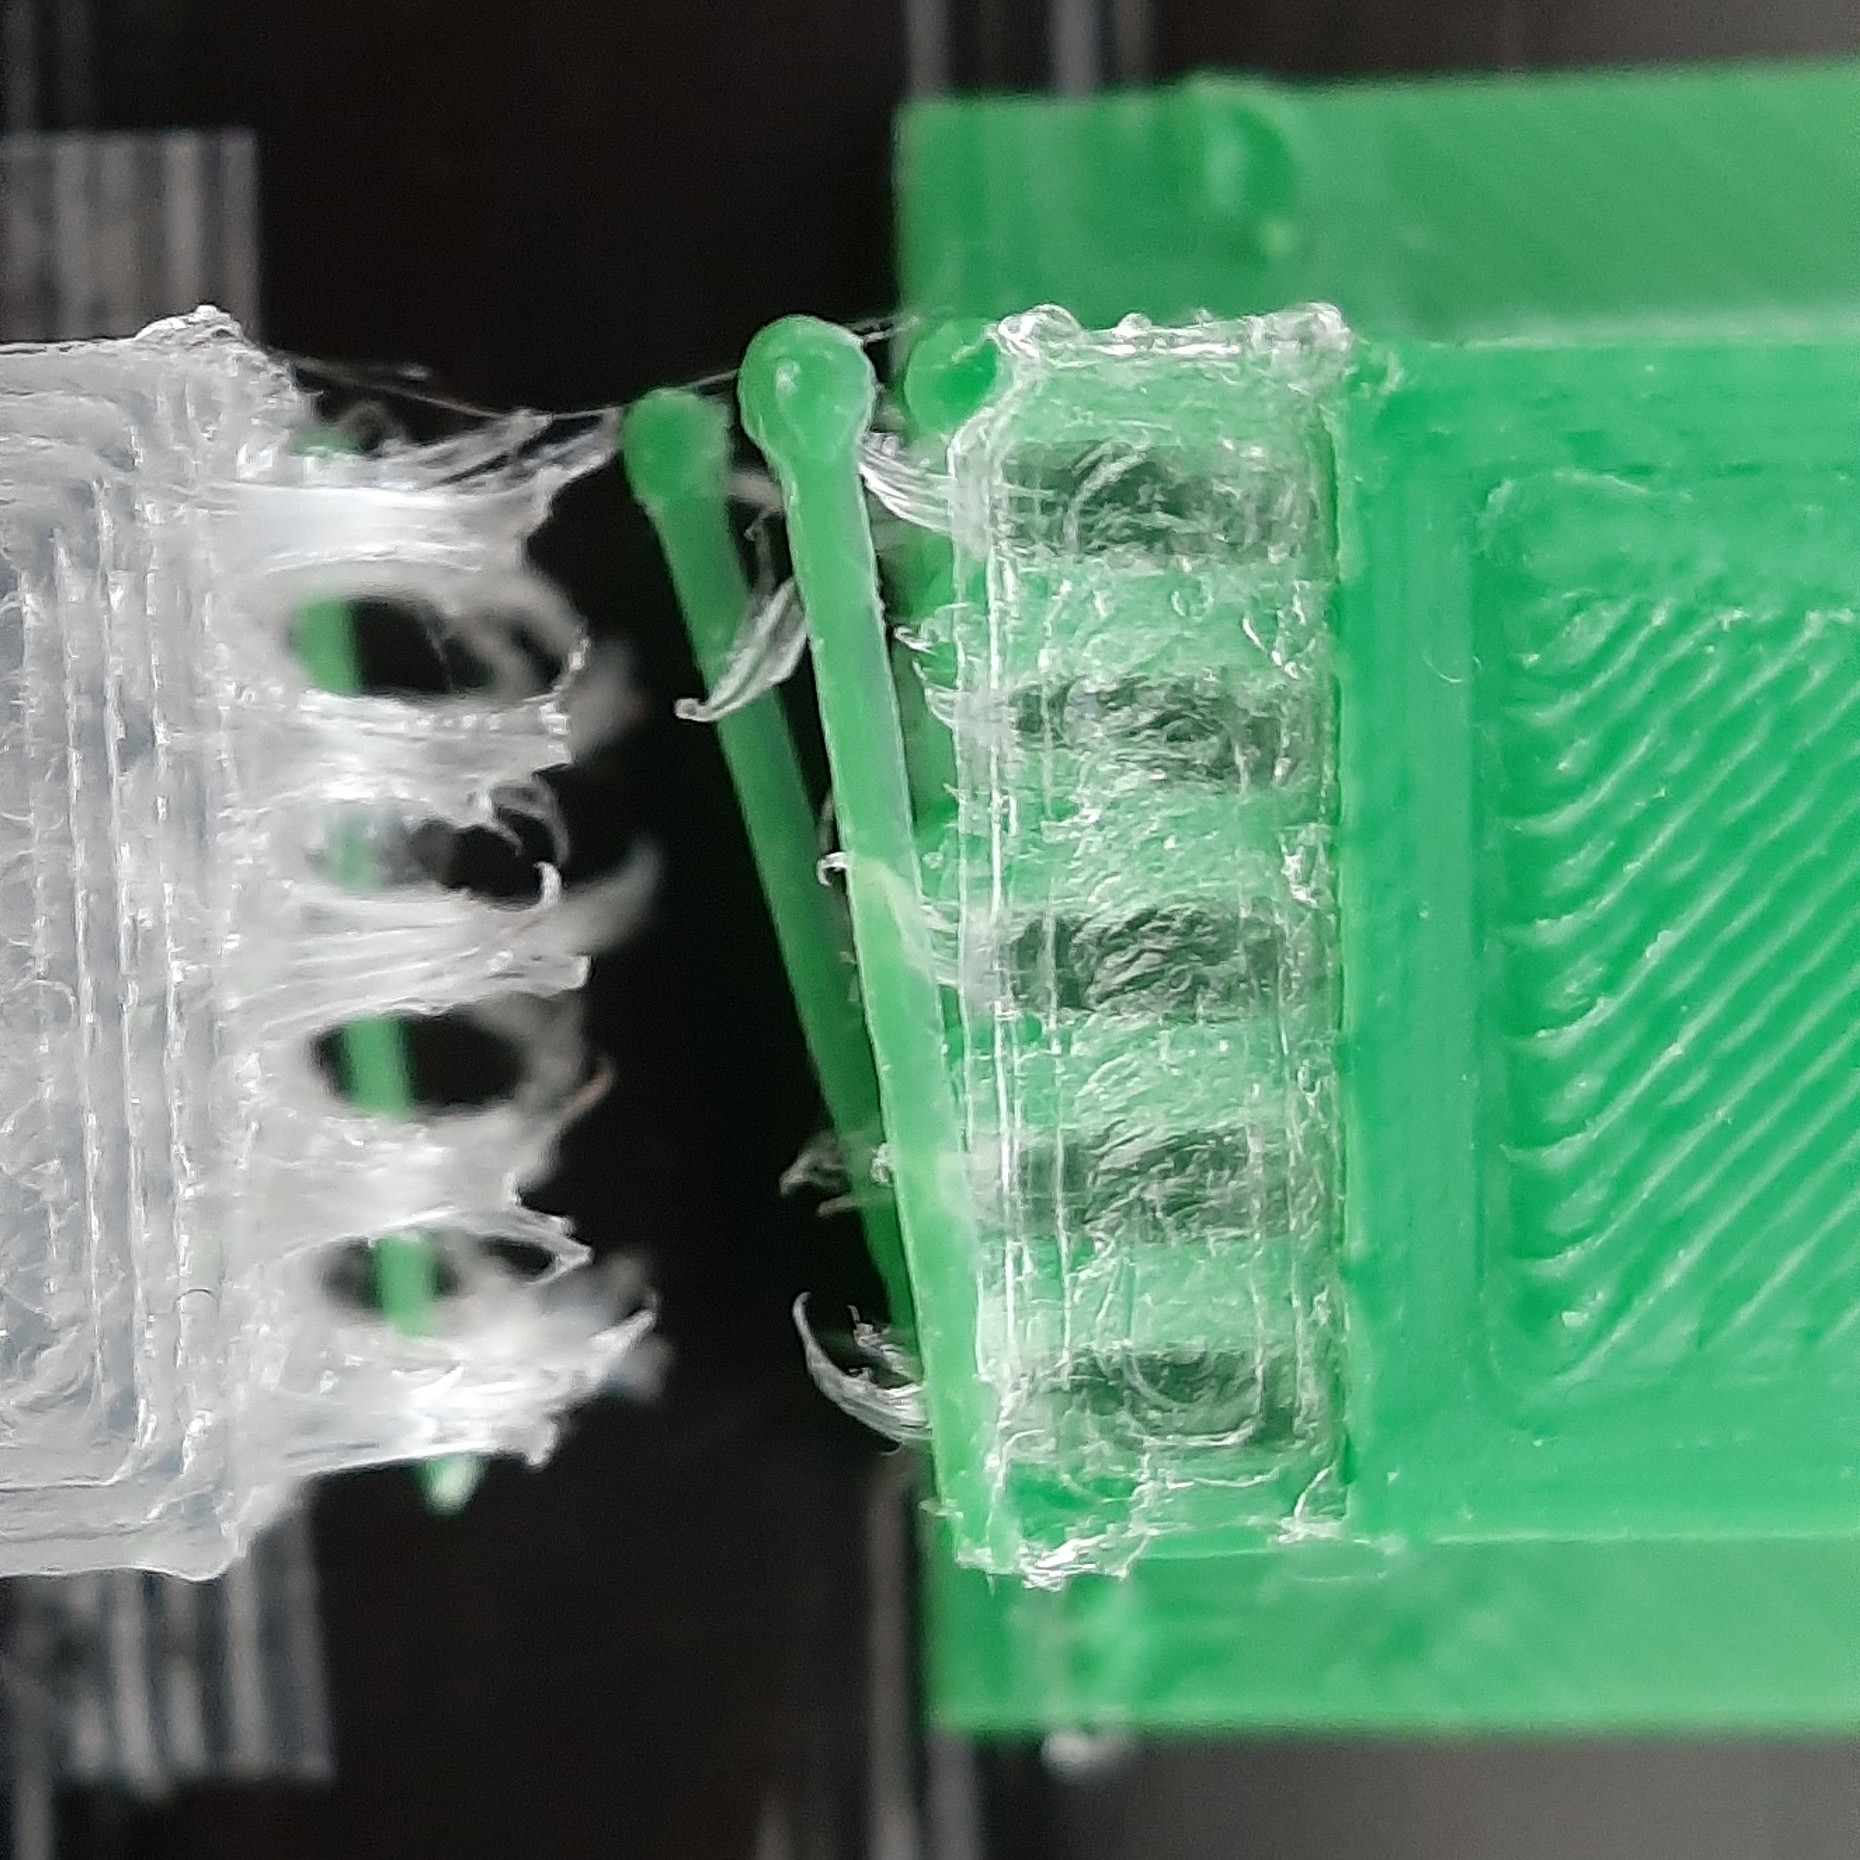
\includegraphics[width=\figwidth]{sources/testing/j5_cropped.jpg}
		\caption{Straight broken wb+}
		\label{fig:failures_straight}
	\end{subfigure}
	\setlength{\figheight}{.25\columnwidth}
	\begin{subfigure}[B]{.28\columnwidth}
		\centering
		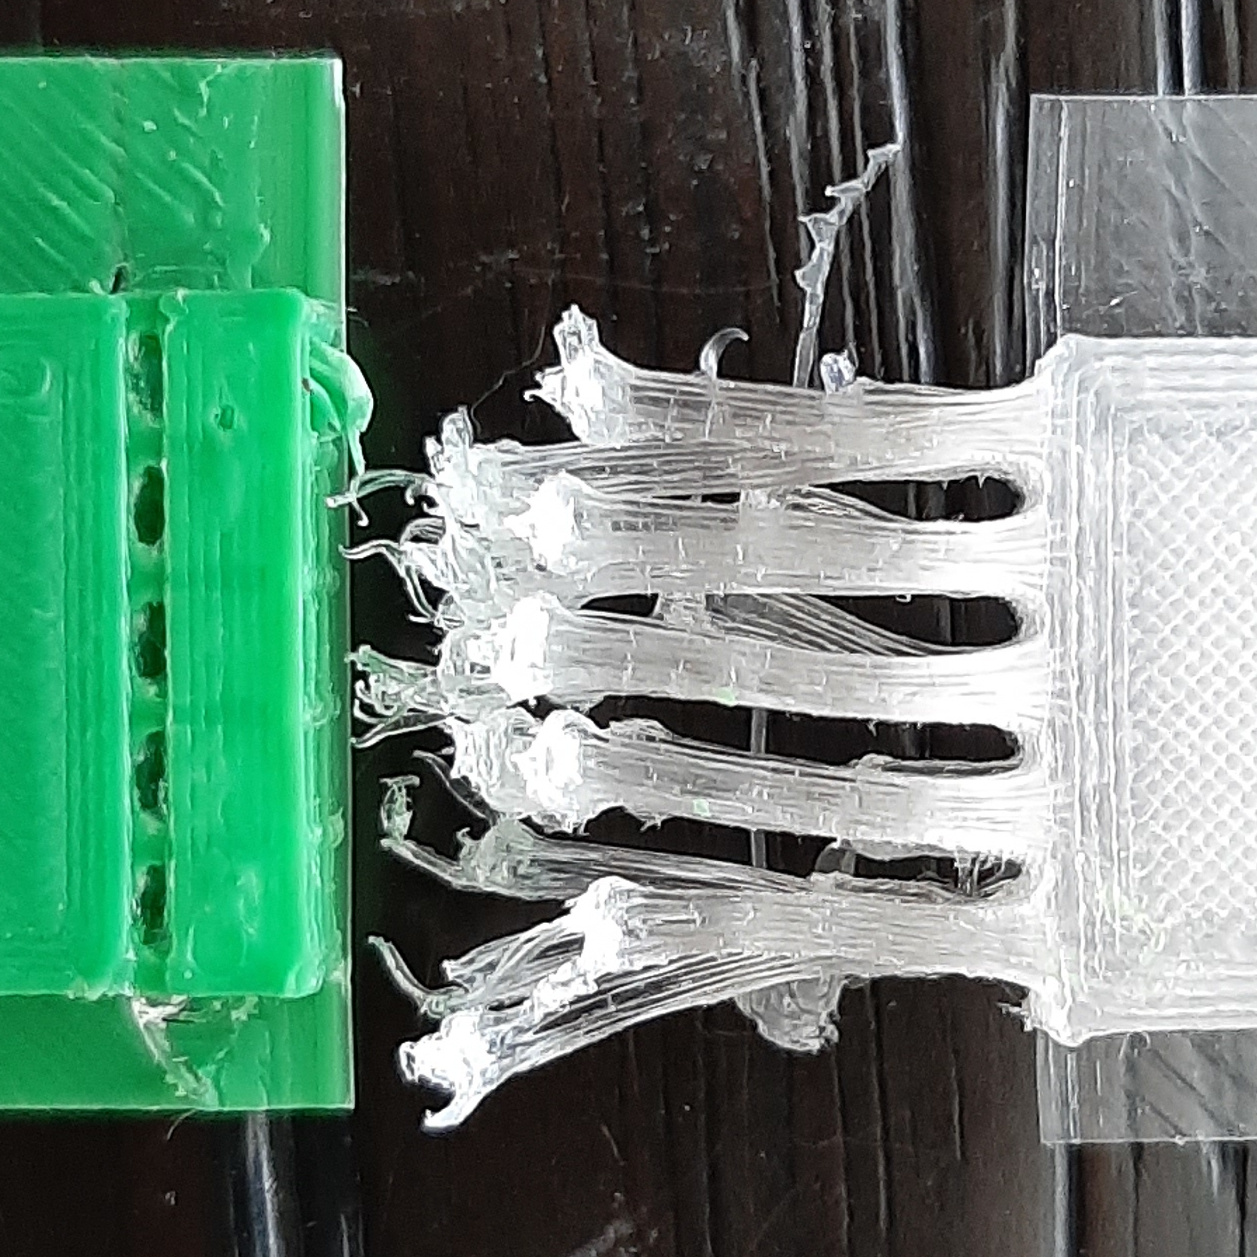
\includegraphics[height=\figheight]{sources/testing/a1_cropped.jpg}
		\caption{Striaght whole}
		\label{fig:failures_whole}
	\end{subfigure}
	\begin{subfigure}[B]{.28\columnwidth}
		\centering
		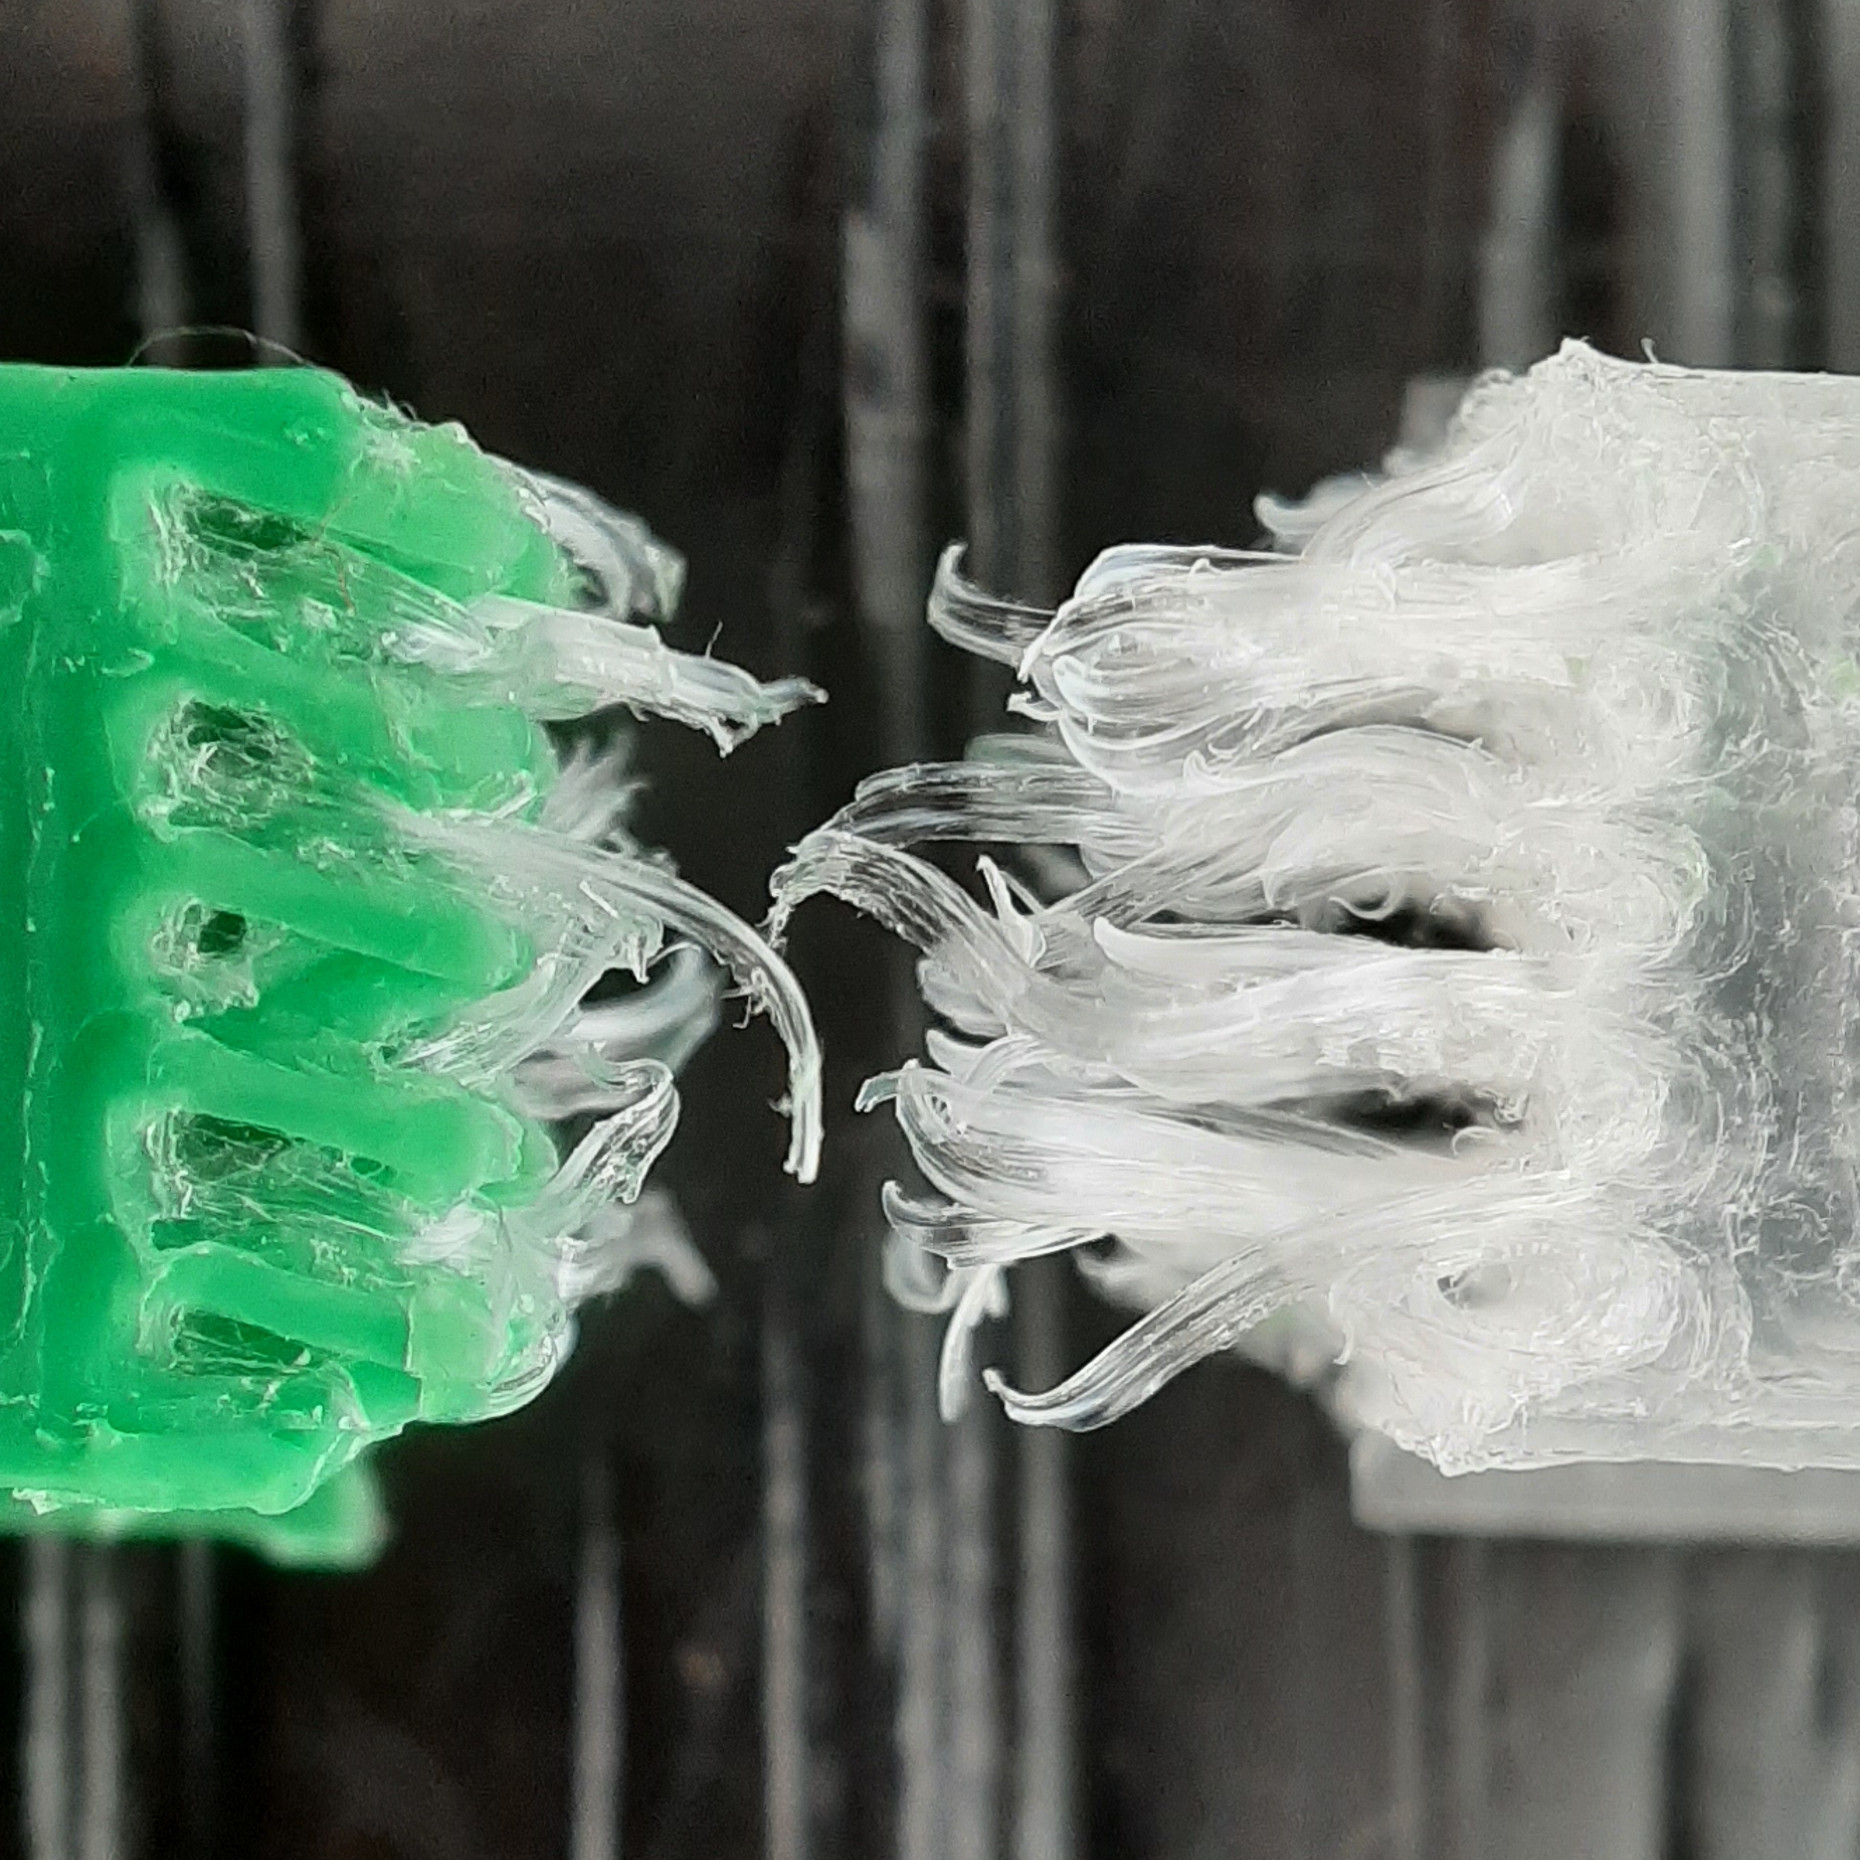
\includegraphics[height=\figheight]{sources/testing/v1_cropped.jpg}
		\caption{Diagonal $1.2$}
		\label{fig:failures_diagonal}
	\end{subfigure}
	\begin{subfigure}[B]{.18\columnwidth}
		\centering
		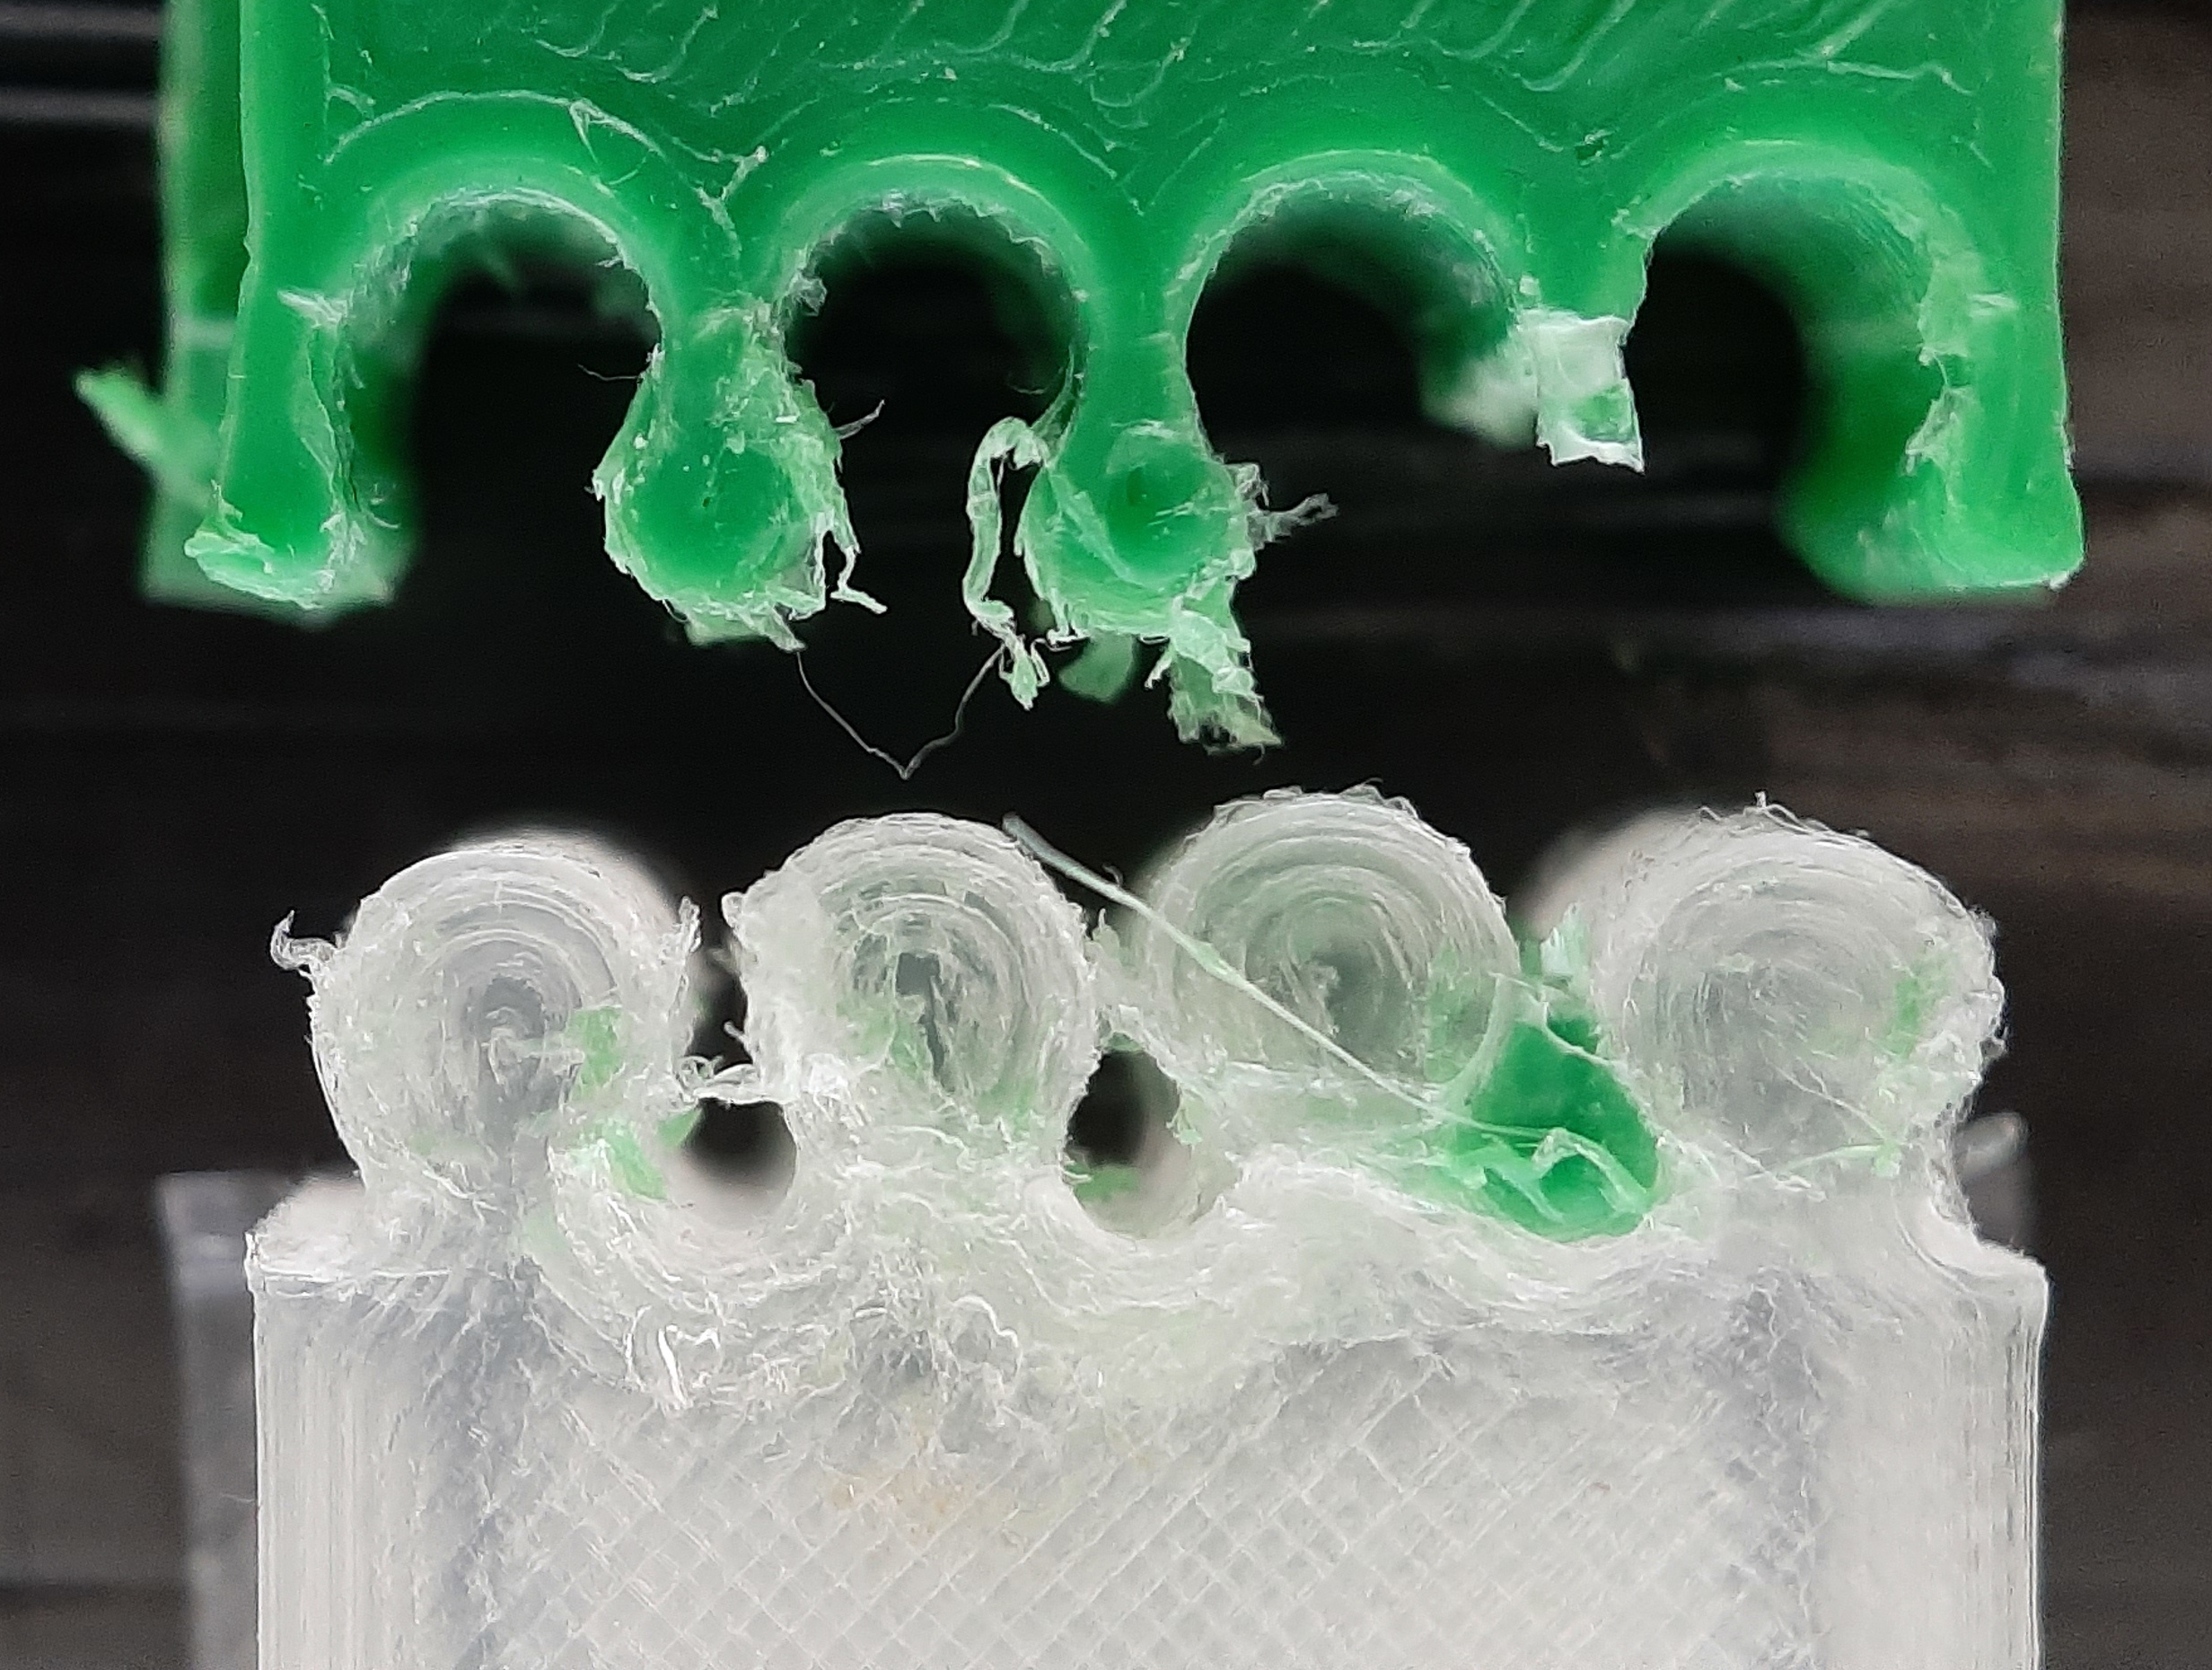
\includegraphics[height=\figheight]{sources/testing/jigsaw_cropped.jpg}
		\caption{Jigsaw $1.8$}
		\label{fig:failures_jigsaw}
	\end{subfigure}
	\begin{subfigure}[B]{.22\columnwidth}
		\centering
		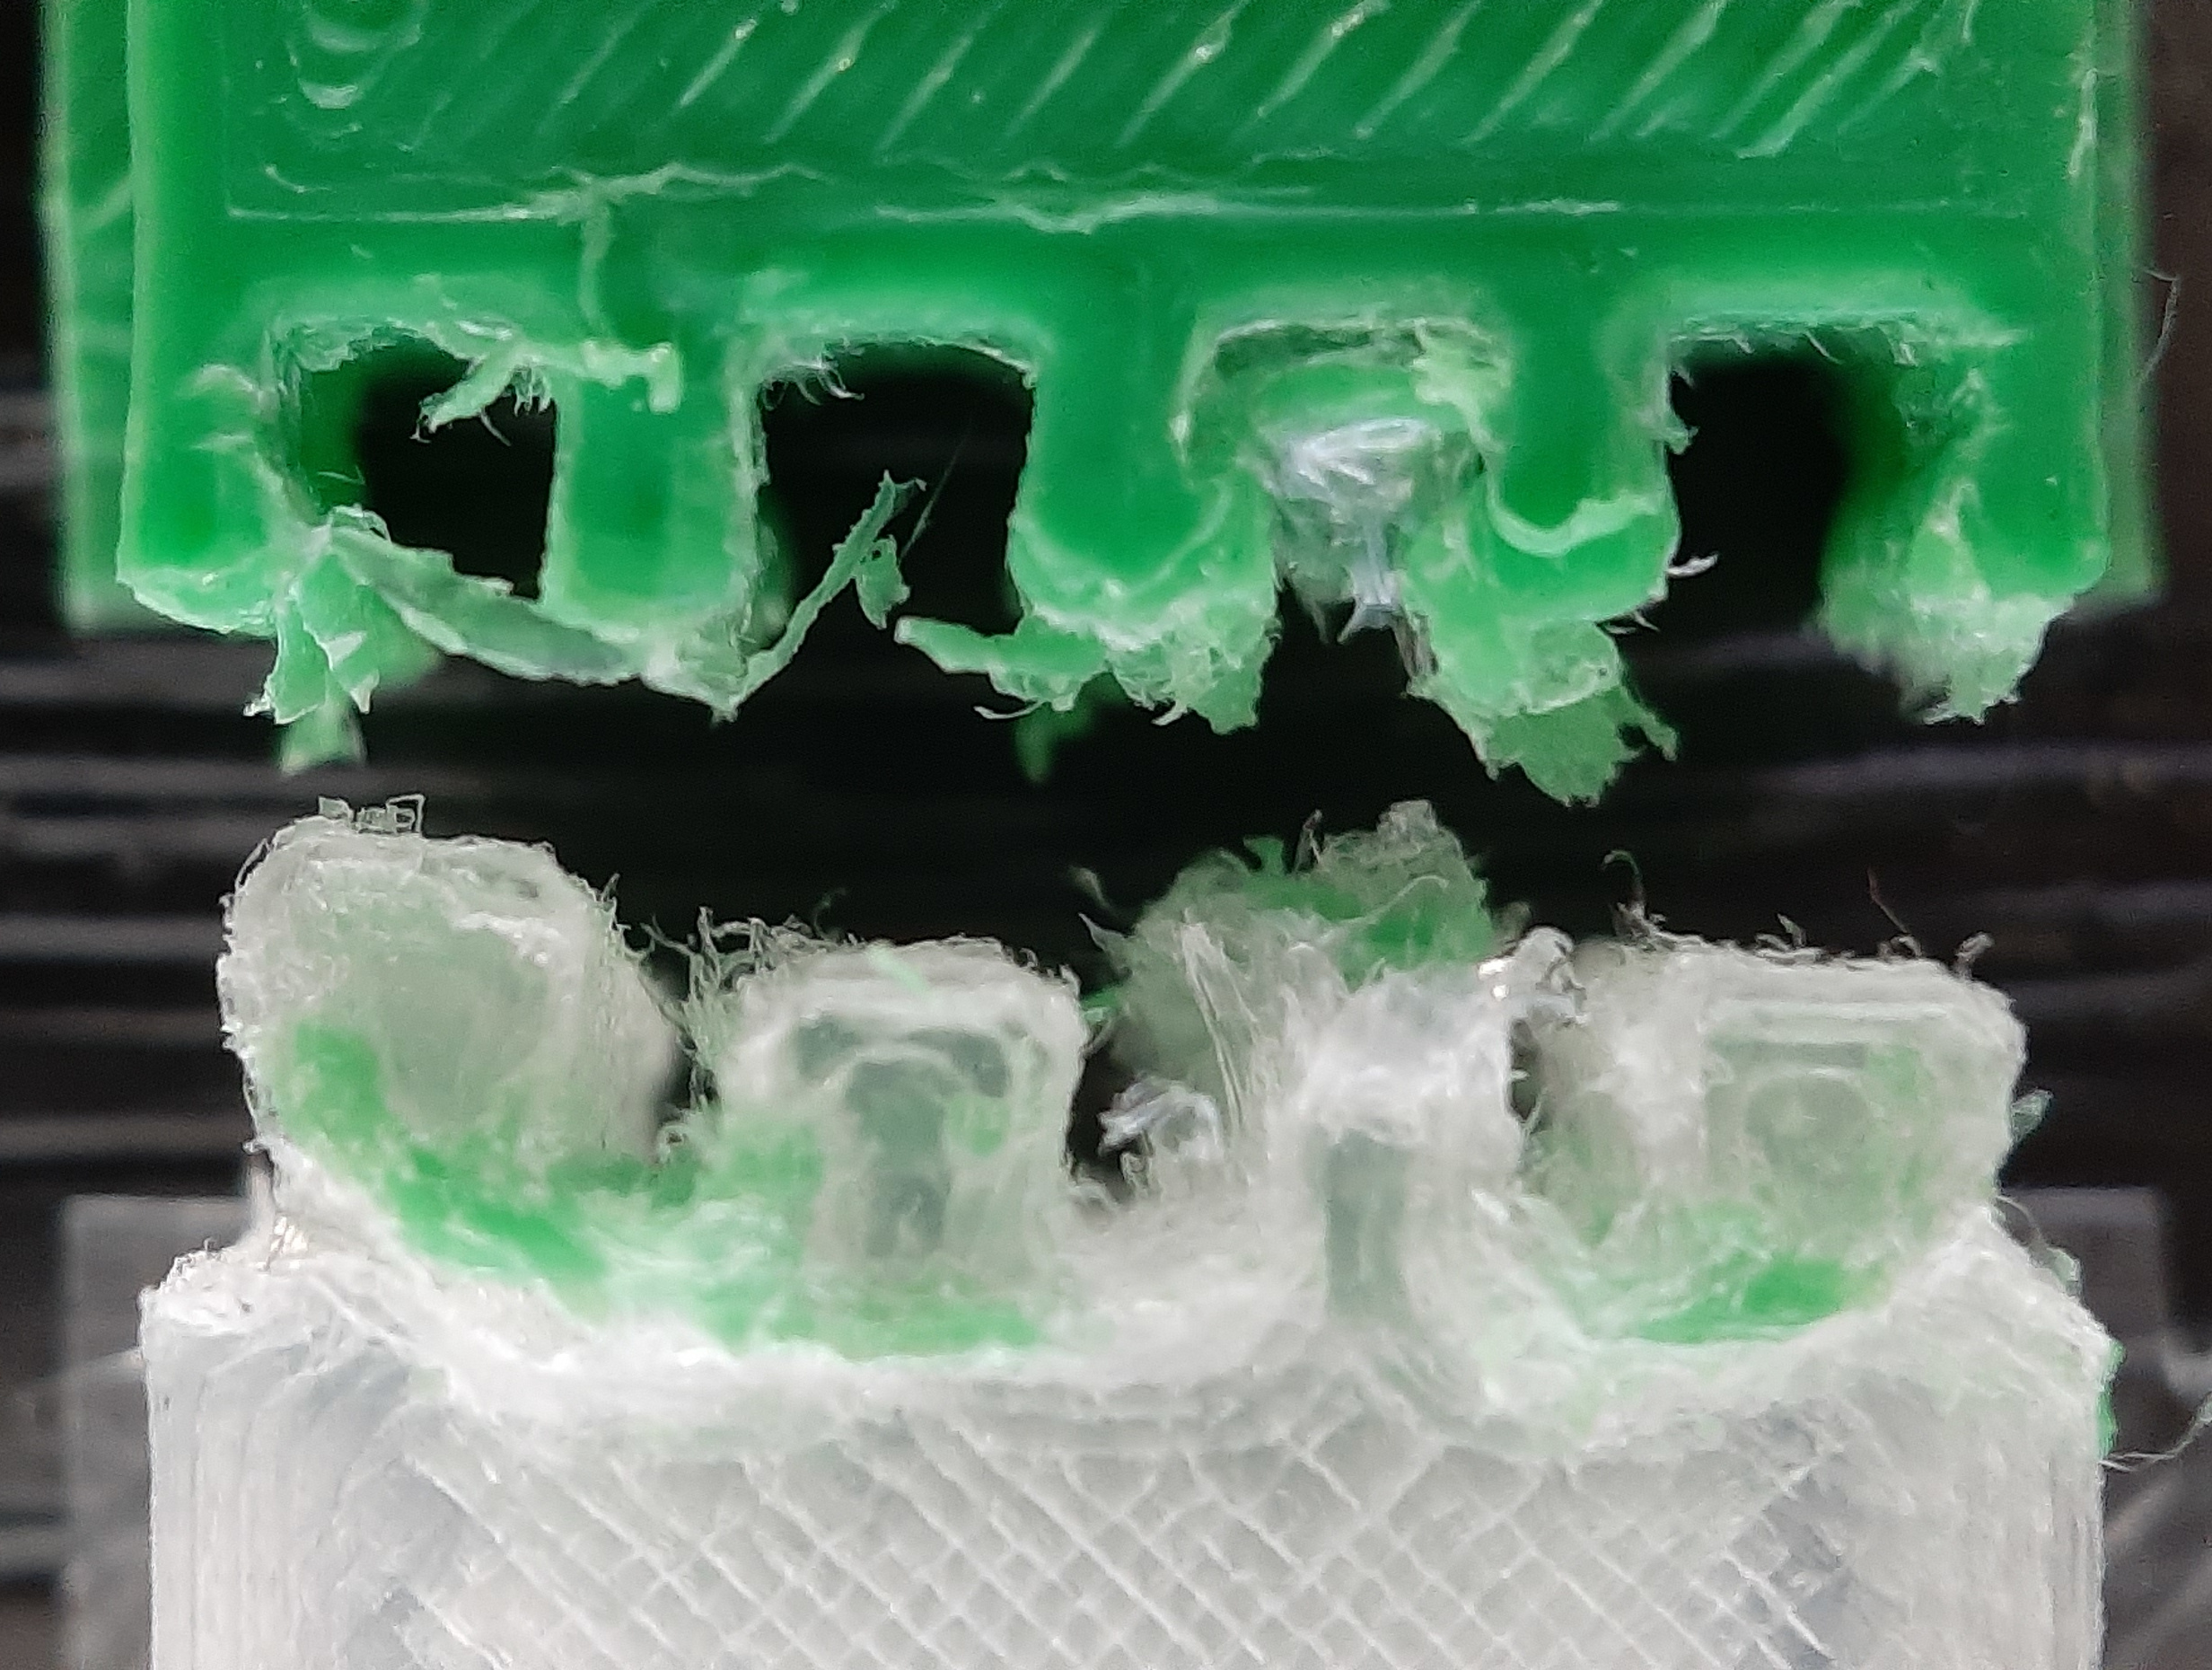
\includegraphics[width=\figheight,rotate=90]{sources/testing/suture_wide_cropped.jpg}
		\caption{Trap. suture $2.7$}
		\label{fig:failures_suture}
	\end{subfigure}
	\caption{Samples after tensile tests of the best performing designs.
		The broken wb+ samples from the straight model exhibit multiple failure modes, indicating that this sample was close to the intersection of several constraint surfaces.}
	\label{fig:failures}
\end{figure}



% table of best sample dimensions?



